\documentclass[11pt]{article}

\usepackage{report}
% \usepackage{sourcecodepro}
\usepackage[utf8]{inputenc} % allow utf-8 input
\usepackage[T1]{fontenc}    % use 8-bit T1 fonts
\usepackage[colorlinks=true, linkcolor=black, citecolor=blue, urlcolor=blue]{hyperref}       % hyperlinks
\usepackage{url}            % simple URL typesetting
\usepackage{booktabs}       % professional-quality tables
\usepackage{amsfonts}       % blackboard math symbols
\usepackage{amsmath}
\usepackage{nicefrac}       % compact symbols for 1/2, etc.
\usepackage{microtype}      % microtypography
\usepackage{lipsum}		% Can be removed after putting your text content
\usepackage{graphicx}
\graphicspath{ {./images/} }
\usepackage{natbib}
\usepackage{doi}
\setcitestyle{aysep={,}}
\usepackage{array}
\usepackage{listings}

\title{CT2108 - Networks \& Data Communications I}

\author{Andrew Hayes\\
\AND
Student ID: 21321503\\
\AND
\AND
\AND
\AND
	2BCT\\
\AND
	University of Galway\\
}

% Uncomment to remove the date
% \date{February 2022}

% Uncomment to override  the `A preprint' in the header
\renewcommand{\headeright}{Networks \& Data Communications I}
\renewcommand{\undertitle}{Networks \& Data Communications I}
\renewcommand{\shorttitle}{}

%%% Add PDF metadata to help others organize their library
%%% Once the PDF is generated, you can check the metadata with
%%% $ pdfinfo template.pdf
% \hypersetup{
% pdftitle={A template for the arxiv style},
% pdfsubject={q-bio.NC, q-bio.QM},
% pdfauthor={David S.~Hippocampus, Elias D.~Striatum},
% pdfkeywords={First keyword, Second keyword, More},
% }
\raggedbottom

\begin{document}
\maketitle

\newpage
\tableofcontents
\thispagestyle{empty}


\newpage
\setcounter{page}{1}
\section{Introduction}
\subsection{Computer Networks}
A \textbf{Computer Network} is a collection of autonomous devices interconnected by some type of network technology. 
Networks come in many shapes \& sizes. 
The Internet is a network of networks - The World Wide Web is not a physical network; It is a distributed \textbf{Client-Server}
application that runs over the Internet.

Two computers are said to be \textbf{interconnected} if they are able to exchange information. 
This connection can be copper wire, optical fiber, wireless, etc. 

\subsubsection{Client-Server Model}
The \textbf{Client-Server} model is employed in most network applications. 
The \textbf{Server} is a powerful machine that can have multiple concurrent \textbf{Clients} accessing its resources at the 
same time. 
Clients are usually simpler devices that run apps to interpret or display information provided by the server. 

\begin{center}
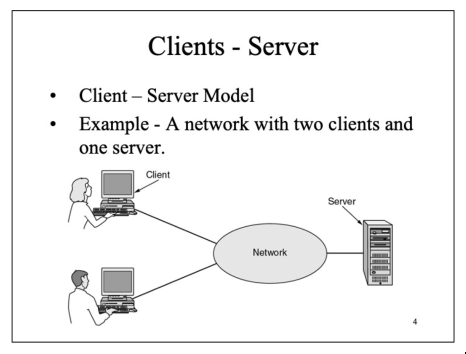
\includegraphics[width=0.5\textwidth]{client-server-example.png}
\end{center}

The client-server model involves requests \& replies. 
It employs at least two process: one running on the server and one running on the client. 

\begin{center}
    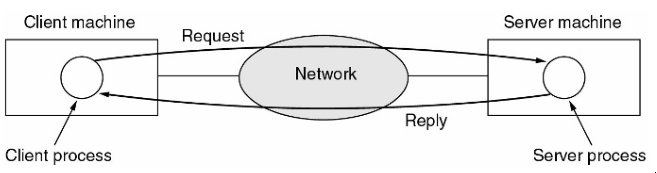
\includegraphics[width=0.7\textwidth]{client-server-diagram.png}
\end{center}

\subsubsection{Home Network Applications}
Home Network applications provide a variety of uses including:
\begin{itemize}
    \item Access to remote information such as newspapers, publications, etc. 
    \item Person-to-person communication such as instant messaging, email, peer-to-peer communication, interactive entertainment, and video on demand. 
    \item Electronic commerce. 
\end{itemize} 

In \textbf{peer-to-peer} systems, there are no fixed clients \& servers. 
Newer P2P systems don't have a centralised database. 
Lookup of the content comes from a local db-s maintained by each of the members. 
Besides content, each user maintains a list of other users as well. 

\subsubsection{Network Types}
Network types include:
\begin{itemize}
    \item Local Area Networks (LAN). 
    \item Metropolitan Area Networks. 
    \item Wide Area Networks. 
    \item Wireless Networks. 
    \item Home Networks. 
    \item The Internet. 
\end{itemize} 

Classification of interconnected processors by scale: 
\begin{center}
    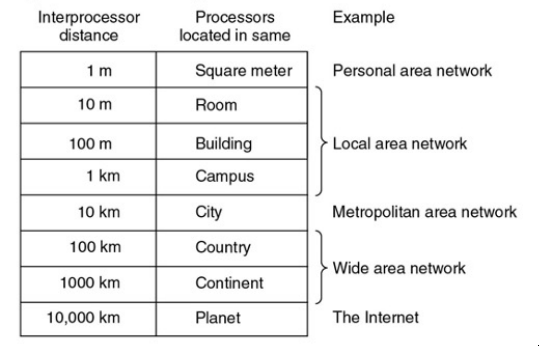
\includegraphics[width=0.7\textwidth]{interconnected-processors-by-scale.png}
\end{center}

\newpage
\subsubsection{Local Area Networks}
\textbf{Local Area Networks} are privately owned networks within a single building or campus, up to a few kilometres in size. 
LANs are restricted in size, so the worst case transmission time is bounded \& known in advance. 

LANs often use the same cable, to which all the machine in the network are attached. 
Speeds generally range from about 100Mb/s to about 10Gb/s. 


Various \textbf{topologies} are possible for broadcast LANs. 
\textbf{Bus}, \textbf{Star} (the most important of which is \textbf{Ethernet}, \& \textbf{Ring} topologies are the most common. 

\textbf{Ethernet} is a bus-based network, with a bus and/or start topology, and is a broadcast decentralised network. 
Ethernet usually operates at about 100Mb/s to 10Gb/s. 
Computers in an Ethernet network can transmit whenever they want. 
If two packets collide, each computer just waits a random amount of time and tries again later.

\begin{center}
    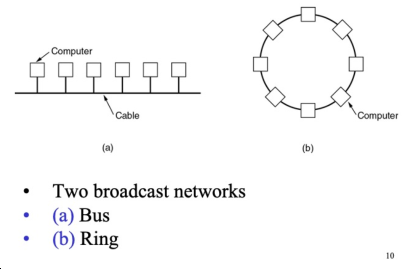
\includegraphics[width=0.7\textwidth]{lan-diagram.png}
\end{center}

\newpage
\subsubsection{Metropolitan Area Networks}
A \textbf{Metropolitan Area Network (MAN)} covers a city. 
One of the most commonly known examples of a MAN is the cable Television Network available in many cities. 
Until the late 1990s these were intended for television only, but cable providers soon realised that they could offer two-way 
Internet in the unused parts of the spectrum. 
This transformed the TV network in a metropolitan area network. 


\begin{center}
    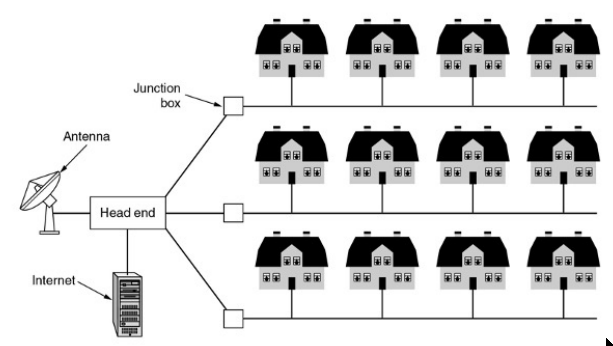
\includegraphics[width=0.7\textwidth]{man-diagram.png}
\end{center}

\subsubsection{Wide Area Networks}
A \textbf{Wide Area Network (WAN)} spans over a large area, often a country or a continent. 
It contains a number of machines called \textbf{hosts} that are connected by a communication \textbf{subnet}.
The hosts are usually owned by individuals, while the subnet is owned by the telecom or Internet providers. 

The job of the subnet is to carry messages from host to host. 
Separation of the pure communication aspects of the network (the subnet) from the application aspects (hosts) simplifies the 
complete network design. 

\textbf{Transmission Lines} move bits between machines. 
They can be copper, optical fiber, radio, etc. 

\textbf{Switching Components} are specialised computers that connect three or more transmission lines. 
When data comes on one of the lines, the switching element must choose an ongoing line to forward the data. 
\textbf{Router} is the technical name for these switching elements. 

\begin{center}
    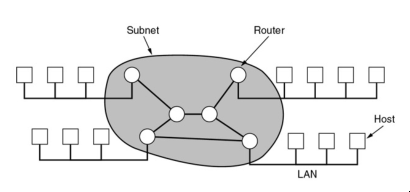
\includegraphics[width=0.7\textwidth]{wan-diagram.png}
\end{center}

A \textbf{store-and-forward} or \textbf{packet switched} subnet is one where the packets are received entirely at intermediate 
routers, stored until some outgoing transmission line is free, and then forwarded to the next router. 
When packets are small \& all the same size, they are called \textbf{cells}. 

When a process on a host wants to send a message to another host in the network, the sending host cuts the message into packets,
each one carrying some sort of sequence number. 
Those packets are then injected into the network one at a time, in quick succession. 
The packets are delivered over the network to the receiving host, where they are re-assembled \& delivered to the receiving process. 

In this figure, all the packets from sender to receiver follow the same route: $ A \rightarrow C \rightarrow E $.
In some subnets, the packets \textit{must} always follow the same path. 
In other subnets, the packets can follow different paths (they are routed separately). 
When the packet is getting to router $A$, the decision to follow path $C$ or path $B$ is made locally. 
This decision is made by and the way in which this decision is made is called the \textbf{routing algorithm}.

\begin{center}
    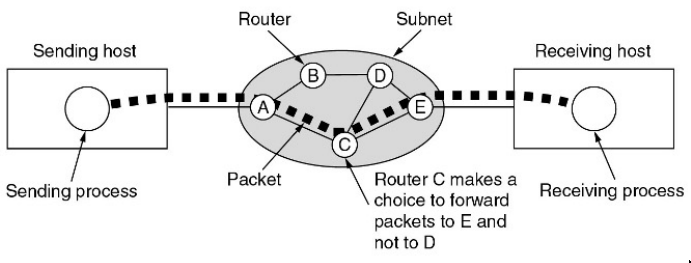
\includegraphics[width=0.7\textwidth]{wan-diagram-2.png}
\end{center}

\subsubsection{Wireless Networks}
\textbf{Bluetooth} is an example of a system interconnection network, and it refers to interconnecting computer components 
(monitor, mouse, keyboard, etc.). 
It is a master-slave topology. 
The master tells the slaves which addresses to use, when they can broadcast, how long they can transmit, what frequencies they 
can use, and other information.

\textbf{Wireless LANs} are networks in which each computer has a radio modem \& antenna with which it can communicate with other
systems. 
IEEE 802.11 is a basic standard for wireless LAN. 
A number of newer, derivative standards are now in place. 

Cellular phone networks such as 3G/4G/5G are examples of \textbf{Wireless WANs} 

\begin{center}
    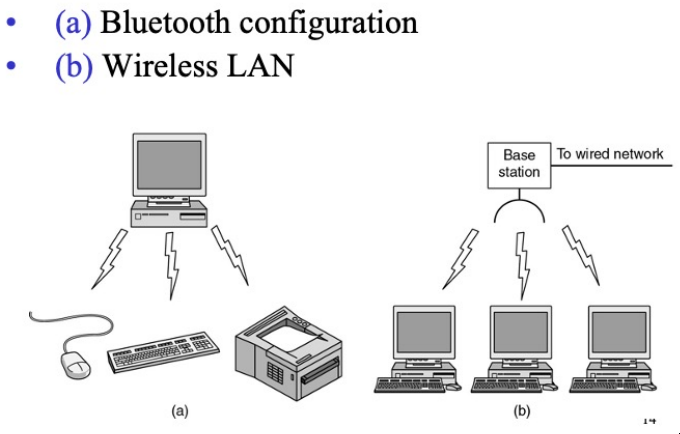
\includegraphics[width=0.7\textwidth]{wlan.png}
\end{center}

\subsection{Network Software}
\subsubsection{Protocol Hierarchies}
To reduce complexity of design, each network is organised as a layer, each one building upon the one below it.
The number of layers, the name of each layer, and the contents \& the function of each layer differ from network to network.

The purpose of each layer is to create services for the layer above, hiding the details of how of those services are actually 
implemented to the those layers. 
The fundamental idea is that a particular piece of software (or even hardware) provides a service to its users but keeps the 
details of its internal state \& algorithms hidden from them. 
Layer $n$ on a machine carries a conversation with layer $n$ on another machine. 
The rules \& conventions used in this conversation are known as Layer $n$ protocol. 

In essence, a \textbf{protocol} is an agreement between the communicating protocols on how communications are to proceed. 
The entities that implement the protocol at different layers levels are called \textbf{peers}. 
It is peers who communicate using a protocol. 

In reality, no data is directly transferred from layer $n$ on one machine to layer $n$ on the other machine. 
In effect, each layer passes data \& control information to the layer below it, until the lowest layer is reached. 
Below Layer 1 id the \textbf{physical medium}, through which the communication occurs. 
Between each pair of adjacent layers is an interface. 
The interface defines which primitive operations \& services the lower layer make available to the upper one.
The most difficult design issue is to define clean interfaces between layers. 

A set of layers \& protocols is called a \textbf{Network Architecture}. 
A Network Architecture has to contain enough information to allow hardware \& software engineers to design hardware \& software 
that would obey the correct protocol. 
A list of protocols used by a certain system, with one protocol per layer, is called a \textbf{Protocol Stack}. 

\begin{center}
    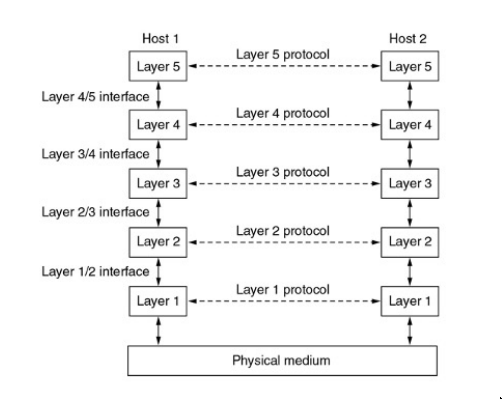
\includegraphics[width=0.7\textwidth]{protocolhierarchies.png}
\end{center}

\newpage
\subsubsection{Protocol Hierarchies Example}
The diagram below shows information flow supporting virtual communication in Layer 5. 

\begin{center}
    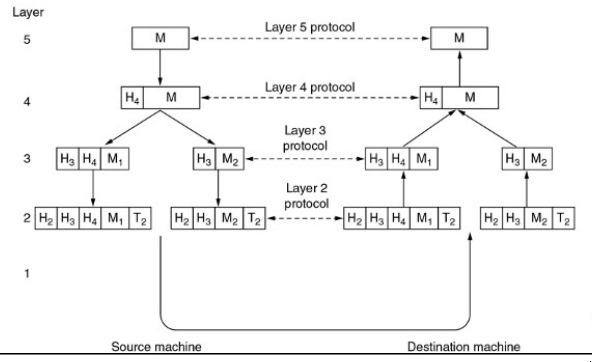
\includegraphics[width=0.7\textwidth]{protocol-hierarchies-example.png}
\end{center}

A message is produced by an application process running at Layer 5. 
Message $M$ is then given to Layer 4 for transmission. 
Layer 4 puts a header in the front of the message to identify the message and passes the result to Layer 3. 
The header includes control information such as sequence numbers to allow Layer 4 in the destination to determine to deliver 
messages in the right order, if the lower layers do not maintain sequence. 
In some layers, headers can also contain sizes, times, \& other control fields. 

At Layer 3, there is a limit on the packet size that can be transmitted. 
Therefore, Layer 3 will break the incoming message into smaller parts called packets, adding header $H3$ corresponding to Layer 3 on each 
packet.
In this example, message $M$ is split into $M1$ \& $M2$. 

Layer 3 decides which outgoing lines to use and passes the message to Layer 2. 
Layer 2 adds not only a header to each piece, but also a trailer, and gives the resulting units to Layer 1 for physical 
transmission. 

At the receiving machine, the message moves upwards, from layer to layer, with headers being stripped off as it progresses. 

\subsubsection{Design Issues for the Layers}
\begin{itemize}
    \item   \textbf{Addressing -} The consequence of having multiple destinations. 
    \item   \textbf{Error Control -} The receiver should be able to inform the sender which data was received correctly. 
    \item   \textbf{Flow Control -} Keep the sender from swamping a slow receiver with data and keep the sender from swamping 
            slow networks with data. 
    \item   \textbf{Multiplexing -} Use the same communications channel for multiple, unrelated conversations.
    \item   \textbf{Routing -} When there are multiple paths between source \& destination, one path must be chosen. 
\end{itemize}

\subsubsection{Connection-Oriented \& Connectionless Services} 
Layers can offer two types of services to the layers above them: connection-oriented services \& connectionless services. 

\textbf{Connection-Oriented Services} are modelled after the phone systems. 
The service users establish connections, use the connections, \& then releases the connection. 
The main idea is that the connection acts as a "pipe" - At one end the data is pushed, and at the other end, data is received. 
In most cases, the order is preserved.
Sometimes, during the connection establishment phase, a \textbf{negotiation} is employed for establishing some parameters of 
the connection. 

Examples of connection-oriented services include:
\begin{itemize}
    \item Reliable message stream (sequence of pages) 
    \item Reliable byte stream (remote login, file transfer, etc.)
    \item Unreliable connection (digitised voice or video). 
\end{itemize} 

\textbf{Connectionless Services} are modelled after the postal system. 
Each message carries the full destination address, each one being routed through the system independent of others. 
It is possible that the messages will arrive at the destination out of order. 

Examples of connectionless services include: 
\begin{itemize}
    \item Datagram service (in analogy with telegram service). 
    \item Acknowledges datagram service. 
    \item Request-reply service. 
\end{itemize}

Each service is characterised by the \textbf{quality of service}. 
Some services are reliable in the sense that they never lose data. 
Usually, reliability is implemented with acknowledgements from the receiver that it received data. 
This introduces overhead \& delays in the communications, which in some cases is fine, but in other is not (e.g. real-time voice \& video communication). 

\subsubsection{Services to Protocols Relationship}
A \textbf{service} is a set of primitives (operations) that a layer provides to the layer above it. 
A service relates to the interface between layers. 

A \textbf{Protocol} is a set of rules governing the format \& meaning of packets exchanged by peer entities within a layer. 
Protocols relate to the packets that are sent between peer entitites between different machienes. 

\begin{center}
    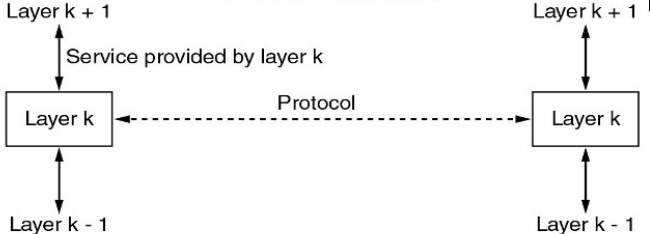
\includegraphics[width=0.7\textwidth]{services-to-protocols-relationship.png}
\end{center}

\newpage
\section{Reference Models}
\subsection{The OSI Reference Model}
The \textbf{Open Systems Interconnect (OSI)} model is a network architecture based on a proposal developed by ISO to standardise 
the protocols used in various layers. 

\begin{center}
    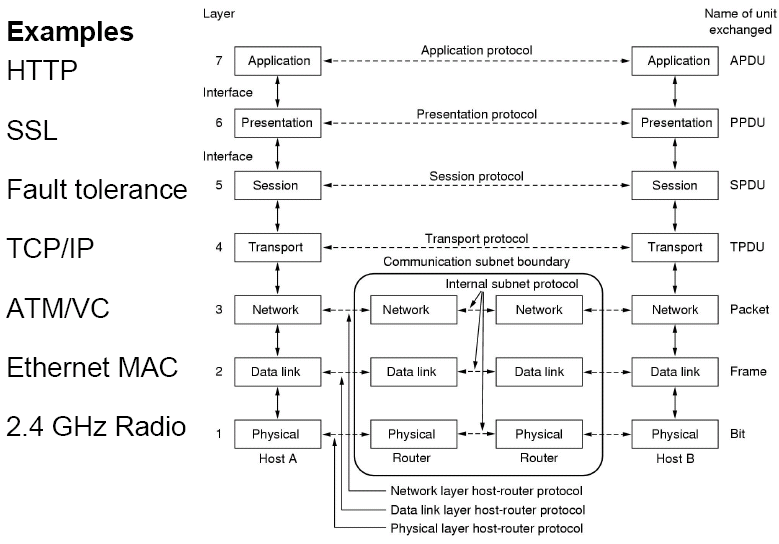
\includegraphics[width=0.7\textwidth]{osimodel.png}
\end{center}

It consists of a seven layer design. The design principles that led to this seven-layer design as follows:
\begin{enumerate}
    \item   A layer should be created where a \textbf{different abstraction is needed}. 
    \item   Each layer should perform a \textbf{well-defined function}. 
    \item   The function of each layer should be chosen with an eye toward defining \textbf{internationally standardised protocols}. 
    \item   The layer boundaries should be chosen to \textbf{minimise the information flow across the interfaces}. 
    \item   The number of layers should be large enough to avoid throwing together separate, \textbf{distinct functions} out of 
            necessity \& small enough to avoid inefficiency. 
\end{enumerate} 

\subsubsection{OSI Layer 1 - The Physical Layer}
The \textbf{Physical Layer} deals with transmitting raw bits over the communication channel. 
It addresses typical questions such as:
\begin{itemize}
    \item   ``How many volts are used to represent a `1' and how many for a `0'?''
    \item   ``How many nanoseconds does a bit last?''
    \item   ``Is there full duplex transmission or not? (Both directions).''
    \item   ``How is the initial connection established and how is it torn down when both sides are finished?''
    \item   ``How many pins will the network connect have and what is each pin used for?''
\end{itemize} 

It deals with design issues such as mechanical, electrical, \& timing interfaces and the physical transmission medium. 
Sending one bit ``1'' on one side must be received on the other side as ``1'' not as ``0''.
        
\subsubsection{OSI Layer 2 - The Data Link Layer}
The purpose of the \textbf{Data Link Layer} is to transform the raw transmission facility (offered by the Physical Layer) into
a line that appears free of undetected transmission errors to the Network Layer. 

It addresses several design issues:
\begin{itemize}
    \item   \textbf{Error Detection \& Correction:} The sender breaks up the input data into \textbf{data frames} (typically a 
            few hundred or thousand bytes) and transmits the frames sequentially. 
            If the service is reliable, the receiver has to confirm the correct receipt of each frame. 
    \item   \textbf{Flow Control:} The flow of data must be controlled to prevent a fast transmitter from drowning a slow 
            receiver in data. 
            Some traffic regulation mechanism is often needed to let the transmitter know how much buffer space the receiver 
            has at the moment. 
            Usually, this is integrated with the error handling mechanism. 
    \item   Broadcast networks have an additional issue in the Data Link Layer: how to control \textbf{access to the shared channel}. 
            A special sub-layer of the data-link layer, the medium access control sub-layer deals with this problem. 
\end{itemize} 

\subsubsection{OSI Layer 3 - The Network Layer} 
The \textbf{Network Layer} controls the operation of the subnet. 

It addresses several design issues:
\begin{itemize}
    \item   \textbf{Routing -} How packets are routed from source to destination. 
    \item   \textbf{Congestion Control -} If too many packets are present in the subnet at the same time. 
    \item   Allow heterogeneous networks to be interconnected. 
    \item   In broadcast networks, the routing problem is thin or non-existent.
\end{itemize} 

\subsubsection{OSI Layer 4 - The Transport Layer}
The \textbf{Transport Layer} accepts data from the above layer (the Session Layer), splits it into smaller units, \& passes 
them to the Network Layer. 
It ensures that these pieces arrive correctly at the other end. 
It also determines what type of service to provide:
\begin{itemize}
    \item   The most popular type of transport connection is an error-free, point-to-point channel which delivers messages or 
            bytes in the order in which they were sent.
    \item   Other types of transport services include delivering datagrams with no guarantee about the order of delivery \&
            broadcasting messages. 
\end{itemize} 

The Transport Layer is a true end-to-end layer, all the way from source to destination. 

The Transport Layer has to perform its function in a way that isolates the upper layers from the inevitable changes in the 
hardware technology. 

Layers 1 to 3 are \textit{chained}, while layers 4 to 7 are \textit{end-to-end} layers. 

\subsubsection{OSI Layer 5 - The Session Layer}
The \textbf{Session Layer} allows users on different machines to establish sessions between them. 
Sessions offer a variety of services, including: 
\begin{itemize} 
    \item   \textbf{Dialog Control -} Keeping track of whose turn it is to transmit. 
    \item   \textbf{Token Management -} Preventing two parties from attempting the same critical operation at the same time. 
    \item   \textbf{Synchronisation -} Marking long transmissions to make sure they can be resumed from where they were when a 
            crash occurred. 
\end{itemize}

\subsubsection{OSI Layer 6 - The Presentation Layer}
The \textbf{Presentation Layer} is not concerned with moving bits around, but with checking the syntax \& semantics of the data 
that is being moved by the layers below. 
In order to make it possible for computers with different data representations to communicate, the data structures to be 
exchanged can be defined in an abstract way, along with a standard encoding to be used on the wire. 
The Presentation Layer manages these abstract data structures and allows higher-level data structures to be defined \& exchanged. 

\subsubsection{OSI Layer 7 - The Application Layer} 
The \textbf{Application Layer} contains a number of different protocols \& applications that are needed by the users. 
A good example of a widely used application protocol is HTTP, which is the basis for the World Wide Web distributed system. 
When a browser wants a page, it sends the name of the page to a web server using a HTTP protocol. 

\subsection{The TCP/IP Reference Model}
The \textbf{Transmission Control Protocol / Internet Protocol (TCP/IP)} is the network architecture that is used by the Internet, 
which is essentially a packet switching network of networks based on a connectionless internetwork layer. 
It consists of 4 layers, excluding the Presentation \& Session layers in the OSI Model. 

\begin{center}
    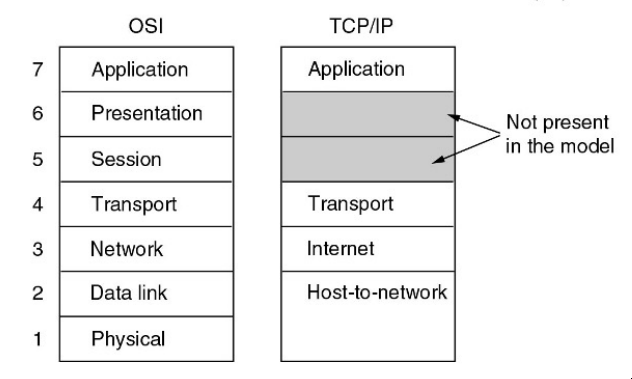
\includegraphics[width=0.7\textwidth]{tcpipmodel.png}
\end{center}

\subsubsection{Layer 1 - The Host-to-Network Layer} 
The \textbf{Host-to-Network Layer} is below the Internet Layer. 
The TCP/IP Reference Model doesn't say much about the Host-to-Network Layer, other than the host has to connect to the network 
using some protocol, so that it can send IP packets to it. 
This protocol is not defined \& varies from host to host and from network to network. 

\subsubsection{Layer 2 - The Internet Layer}
The \textbf{Internet Layer} permits the hosts to inject packets into any network and have them travel independently to the 
destination (potentially using different paths or networks). 
The packets may arrive in a different order. 
It is the job of the higher layer to rearrange them. 

The Internet Layer defines an official packet format \& protocol, called the \textbf{Internet Protocol (IP)}. 
The purpose of the Internet Layer is to deliver IP packets to where they want to go. 
The two biggest issues for the Internet Layer are packet routing and avoiding congestion. 

\subsubsection{Layer 3 - The Transport Layer} 
The \textbf{Transport Layer} is designed to allow peer entities on the source \& destination to carry out a conversation. 

It has two end-to-end protocols: TCP \& UDP. 
\begin{itemize}
    \item   \textbf{Transmission Control Protocol (TCP):} End-to-end, reliable connection-oriented protocol that allows a byte 
            stream originating from one machine to be delivered with no error on another machine in the Internet. 
    \item   \textbf{User Datagram Protocol (UDP):} Unreliable, connectionless protocol for applications that don't want TCP's 
            sequencing flow control and want to provide their own (or for apps that don't want connection overhead). 
\end{itemize}

\subsubsection{Layer 4 - The Application Layer} 
The \textbf{Application Layer} contains all the high level protocols: HTTP, file transfer, e-mail, Domain Name System, etc. 

\begin{center}
    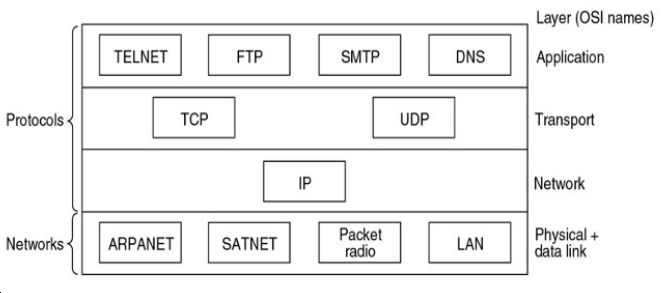
\includegraphics[width=0.8\textwidth]{applicationlayer.png}
\end{center}

\subsection{OSI vs TCP/IP}
The OSI and TCP/IP models have a lot in common. 
Both are based on a concept of stack with independent protocols. 
Additionally, the functionality of the layers is somewhat similar. 


The concepts of \textbf{Services}, \textbf{Interfaces}, \& \textbf{Protocols} are central to the OSI model. 
These three protocols are perhaps the biggest contribution that OSI made.
\begin{itemize}
    \item   \textbf{Services} tell what a certain layer does, not how the entities above it access it, nor how the layer works. 
            It defines the layer's semantics. 
    \item   \textbf{Interfaces} tell the processes above the layer how to access it. 
            An interface specifies the parameters \& what results to expect. 
            Interfaces say nothing about how the layer works internally. 
    \item   \textbf{Protocols} are the business of the peer layers. 
            A layer can use any protocol so long as it gets the job done (i.e., provides the offered services). 
            The protocols can change without affecting the software in the highest layer.
\end{itemize}

TCP/IP did not originally make a clear distinction between services, interfaces, \& protocols. 
Some people have attempted to retrofit services, interfaces, \& protocols after the specifications to make it look more like 
OSI. 
The only real services offered by the IP layer are \verb|SEND_IP_PACKET| \& \verb|RECEIVE_IP_PACKET|. 
Consequently, protocols in the OSI model are better hidden than in the TCP/IP model and can be replaced a lot more easily (as 
the technology changes), without disturbing the layers above. 

The OSI reference was described before the protocols were invented, so the model is not biased towards a set of protocols, and 
is instead rather generic. 
The downside of this is that the designers did not have much experience of which function to put in which layer, etc. 

In TCP/IP, the protocols came first. 
The TCP/IP model was just done as a description of these protocols, so naturally, the protocols fit perfectly to the model. 
The problem with this is that the model does not fit any other protocols, and is useless to describe any other type of model 
that is not TCP/IP based. 

OSI has 7 layers, while TCP/IP has only 4. 

The OSI model supports connectionless \& connection-oriented services at the network layer, but only supports one type of 
connection oriented service at the transport layer. 

The TCP/IP model only supports connectionless services at the network layer, but offers both connection-oriented \& connectionless 
services at the transport layer, giving the users a choice. 

\subsubsection{Problems with the OSI Model \& Protocols} 
The OSI model was never widely adopted, due in part to it's poor timing (the TCP/IP model was already in use when it was established) 
but mainly because of its poor technology \& implementation. 

The Session \& Presentation layers in OSI are nearly empty, while others, like the Network \& Data-Link layers, are overcrowded. 
The OSI protocols \& service definitions are very complex, bordering on incomprehensible. 
Some of the functions in OSI (such as addressing, flow control, \& error control) reappear again \& again at different layers, 
which is unnecessary \& inefficient. 

Given the complexity of the protocols, the implementations were huge \& inefficient. 
People began to associate OSI with poor quality because the implementations were so slow on the available equipment. 
In contrast, one of the first implementations of TCP/IP was part of Berkeley's UNIX and was quite good, as well as being free. 

\subsubsection{Problems with the TCP/IP Model \& Protocols} 
\begin{itemize}
    \item Service, interface, \& protocol not distinguished. 
    \item Not a general model. 
    \item The host-to-network layer is not really a layer. 
    \item No mention of physical \& data link layers. 
    \item Minor protocols are deeply entrenched, hard to replace. 
\end{itemize}

\newpage
\subsection{The Hybrid Model}
The \textbf{Hybrid Model} will be used in this course. 

\begin{center}
    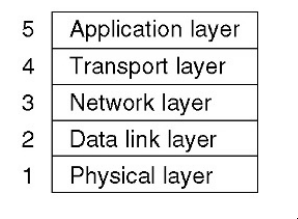
\includegraphics[width=0.3\textwidth]{hybridmodel.png}
\end{center}

\section{The Theoretical Basis for Data Communication \& the Physical Layer}
\subsection{Fourier Analysis}
A periodic signal with period $T$ can be constructed as a sum of several sines \& cosines. 

\[
    g(t) = \frac{1}{2}c + \sum^\infty_{n=1} a_n \text{sin}(2\pi n f t) + \sum^\infty_{n=1} b_n \text{cos} (2 \pi n f t) 
\]

Where: 
\begin{itemize}
    \item $f = \frac{1}{T}$.
    \item $a_n$ \& $b_n$ are the sine \& cosine amplitudes of the $n^{th}$ harmonics. 
    \item $c$ is a constant. 
\end{itemize}

Such a decomposition is called a \textbf{Fourier Series}.
The original function of time can be reconstructed (by performing the sum) if the period $T$ is known and the amplitudes $a_n$, $b_n$, and the constant $c$ are given. 

The $a_n$ amplitudes can be computed for any $g(t)$ by multiplying the Fourier series by $sin(2 \pi k f t)$ and integrating from $0$ to $T$. 
\[ 
    a_n = \frac{2}{T} \int^T_0 g(t)\text{sin}(2 \pi n f t)dt
\] 

The $b_n$ amplitudes can be computed by multiplying the Fourier series by $cos(2 \pi k f t)$ and integrating from $0$ to $T$. 
\[
    b_n = \frac{2}{T} \int^T_0 g(t)\text{cos}(2 \pi n f t)dt
\]

The constant $c$ can be computed by simply integrating from $0$ to $T$. 
\[
    c = \frac{2}{T} \int^T_0 g(t)dt 
\] 

\newpage
\subsection{Bandwidth-Limited Signals} 
Consider the ASCII character ``b'' encoded in a byte. 
The bit pattern to be sent is \verb|01100010|. 
The way to deal with a data signal that has a fixed duration (like in our example) is to imagine that the entire pattern repeats over \& over again endlessly. 

\begin{center}
    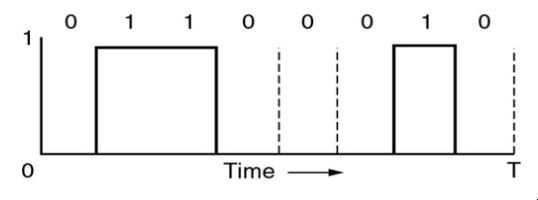
\includegraphics[width=0.7\textwidth]{b.png}
\end{center}

The Fourier analysis of the signal yields the coefficients: 
\begin{center}
    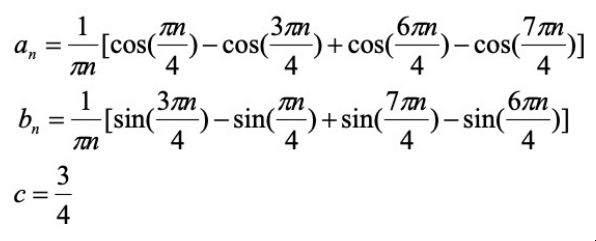
\includegraphics[width=0.5\textwidth]{fouriercoefficients.png}
\end{center}

The \textbf{root mean square (RMS)} amplitudes are of interest because those values show the \textit{energy} transmitted at the corresponding frequency. 
No transmission facility can transmit signals without losing some power in the process. 
If all Fourier components were equally diminished, then the resultant signal would be reduced in amplitude, but not distorted. 
Unfortunately, all transmission media diminish different Fourier components by different amounts, resulting in a distortion of the signal at the receiving end. 

Usually, the amplitudes are transmitted undiminished between $0$ \& a frequency $Fc$ (\textbf{F cut}, measured in Hz), with
all frequencies above this $Fc$ attenuated. 
The range of frequencies being attenuated is called the \textbf{bandwidth}. 
In practice, the cut of frequency is not really sharp, so usually, this bandwidth is the range from $0$ to the frequency where 
half of the power of the signal gets through. 

The bandwidth is a physical property of the transmission medium, and usually depends on the construction, thickness, \& length 
of the medium. 
Consider our signal ASCII ``B'', shown in figure (a) below. 
Look at how the signal would look if only the lowest frequencies were transmitted (i.e., if the function was approximated by only a few terms). 

\begin{center}
    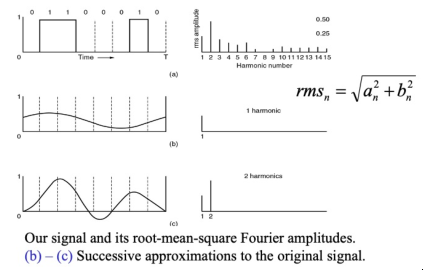
\includegraphics[width=0.7\textwidth]{rms1.png}
\end{center}

\begin{center}
    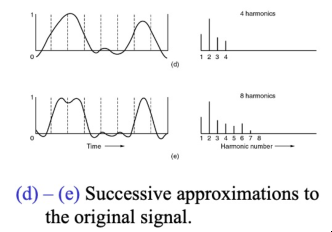
\includegraphics[width=0.6\textwidth]{rms2.png}
\end{center}

Given a rate of $b$ bits per second, the time to send one byte is $\frac{8}{b}$, which is the period for the first harmonic. 
The frequency of the first harmonic would be $\frac{b}{8}$ Hz. 

\begin{center}
    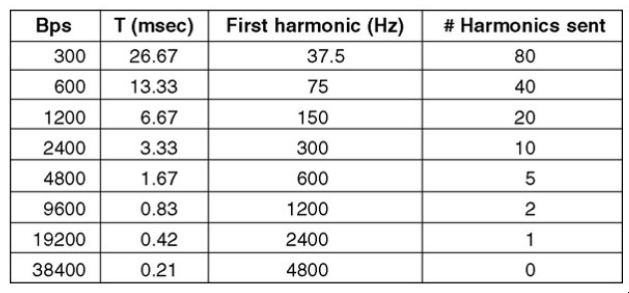
\includegraphics[width=0.7\textwidth]{bps.png}
\end{center}

\subsection{Maximum Data Rate of a Channel}
For a \textbf{noiseless channel}, we determine the maximum data rate with the \textbf{Nyquist Theorem}: 
\[ 
    \text{MaxDataRate} = 2B \text{log}_2V  \text{    [bits/sec]}
\] 
Where:
\begin{itemize}
    \item $B$ is the bandwidth of the noiseless channel. 
    \item $V$ is the number of discrete levels of the signal transmitted through the channel. 
\end{itemize}

If random noise is present, then the situation deteriorates rapidly. 
In reality, there is always random noise, due to the motion of the molecules in the system. 
The amount of thermal noise is measured by the ratio of the signal power to the noise power, called the \textbf{signal-to-noise ratio}: 
\[
    \text{SNR}_{\text{dB}} = 10\text{log}_{10} \left(\frac{S}{N} \right) \text{    [dB]}
\]

The signal to noise ratio is given in \textbf{decibels (dB)} and the ratio itself is not usually quoted. 
A ratio of 10 is 10dB, a ratio of 100 is 20dB, a ratio of 1000 is 30dB, and so on. 

\textbf{Shannon's Theorem}:
\[
    \text{MaxDataRate} = B \text{log}_2 \left( 1 + \frac{S}{N} \right) \text{    [bits/sec]}
\] 
Where:
\begin{itemize} 
    \item $B$ is the bandwidth of the noisy channel. 
    \item $\frac{S}{N}$ is the signal-to-noise ratio of the channel. 
\end{itemize} 

Shannon's Theory demonstrates that the maximum data rate through a channel is limited by the amount of noise present, no matter 
how many or how few signal levels are used and no matter how frequently or infrequently samples are taken. 
This limit is the upper limit, and real systems rarely achieve it. 

\subsection{Channel Organisation}
Any communications channel has a \textit{direction} associated with it. 

\begin{center}
    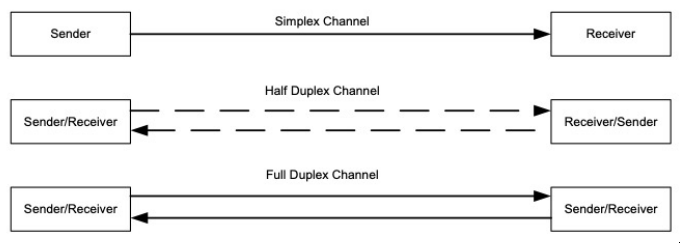
\includegraphics[width=0.8\textwidth]{channelorganisation.png}
\end{center}

The message source is the transmitter, and the destination is the receiver. 
A channel whose direction of transmission is unchanging is referred to as a \textbf{simplex channel}. 
For example, a radio station is a simplex channel because it always transmits the signal to its listeners and never allows them 
to transmit back. 

A \textbf{half-duplex channel} is a single physical channel in which the direction may be reversed. 
Messages may flow in two directions, but never at the same time in a half-duplex system. 

A \textbf{full-duplex channel} allows simultaneous message exchange in both directions. 
It really consists of two simplex channels: a forward channel \& a reverse channel, linking the same points. 
The transmission rate of the reverse may be slower if it is used only for flow control of the forward channel. 

\subsubsection{Synchronisation}
Data is not generally sent at a uniform rate through a channel. 
Instead, there is usually a burst of data followed by a pause, after which the data flow resumes. 
Packets of binary data are sent in this manner, possibly  with variable-length pauses between packets, until the message has been 
fully transmitted. 
In order for the receiving end to know the proper moments to read individual binary bits from the channel, it must know exactly when 
a packet begins and how much time elapses between bits. 
When this timing information is known, the receiver is said to be \textbf{synchronised} with the transmitter, and accurate data 
transfer becomes possible. 
Failure to remain synchronised throughout a transmission will cause data to be corrupted or lost. 
\begin{itemize}
    \item The receiver should know the exact moment when the data is valid. 
\end{itemize}

Two basic techniques are employed to ensure correct Synchronisation: \textbf{synchronous} \& \textbf{asynchronous} communication. 

In \textbf{synchronous systems}, separate channels are used to transmit data \& timing information. 
The timing channel transmits clock pulses to the receiver. 
Upon receipt of a clock pulse, the receiver reads the data channel and latches the bit value found on the channel at that moment. 
The data channel is not read again until the next clock pulse arrives. 
Because the transmitter originates both the data \& the timing pulses, the receiver will read the data channel only when told 
to do so by the transmitter (via the clock pulse), and synchronisation is guaranteed. 
Techniques exist to merge the timing signal with the data so that only a single channel is required. 
This is especially useful when synchronous transmissions are to be sent through a modem. 
Two methods in which a data signal is self-timed are: non-return-to-zero \& bi-phase Manchester coding. 
These both refer to methods for encoding a data stream into an electrical waveform for transmission. 
\begin{itemize}
    \item Data \& timing information are sent separately (through separate channel or the same channel). 
    \item The timing channel transmits clock pulses to the receiver. 
    \item Upon receipt of a clock pulse, the receiver reads the data \& latches it. 
    \item The data is not read again until the next clock pulse arrive. 
\end{itemize}

In \textbf{asynchronous systems}, a separate timing channel is not used. 
The transmitter \& receiver must be preset in advance on timings. 
A very accurate local oscillator within the receiver will then generate an internal clock signal that is equal to the transmitter's 
within a fraction of a percent. 
For the most common serial protocol, data is sent in small packets of 10 or 11 bits, eight of which constitute message information. 
When the channel is idle, the signal voltage corresponds to a continuous logic ``1''. 
A data packet always begins with a logic ``0'' (the start bit) to signal to the receiver that a transmission is starting. 
The start bit triggers an internal timer in the receiver that generates the needed clock pulses. 
Following the start bit, eight bits of message data are sent bit by bit at the upon baud rate. 
The packet is concluded with a parity bit \& a stop bit. 
\begin{itemize}
    \item No separate timing information is used. 
    \item The transmitter \& receiver must agree in advance on timings. 
    \item Start \& stop conditions are used. 
    \item Accurate oscillators will measure the bit widths. 
\end{itemize}

\subsubsection{Parallel Communication}
\begin{enumerate}
    \item   Sender places data on the channel. 
    \item   Sender asserts ``data available''. 
    \item   Receiver reads the data and asserts ``ready'' signal. 
    \item   Sender de-asserts ``data available'' and it will be ready for a new data transfer. 
\end{enumerate}

\begin{center}
    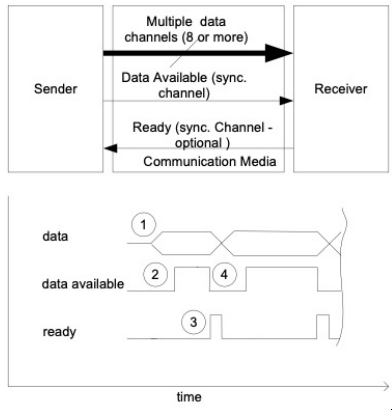
\includegraphics[width=0.45\textwidth]{parallelcomm.png}
\end{center}

\subsubsection{Serial Communication} 
In \textbf{synchronous systems}, separate channels are used to transmit data \& timing information. 
The timing channel transmits clock pulses to the receiver. 
Upon receipt of a clock pulse, the receiver reads the data channel \& latches the bit value found on the channel at that moment. 
The data channel is not read again until the next clock pulse arrives. 
Because the transmitter originates both the data \& the timing pulses, the receiver will read the data channel only when 
told to do so by the transmitter (via the clock pulse) , and synchronisation is guaranteed.

Techniques exist to merge the timing signal with the data so that only a single channel is required. 
This is especially useful when synchronous transmissions are to be sent through a \textbf{modem}. 
Two methods in which a data signal is self-timed are non-return-to-zero and bi-phase Manchester coding. 
These both refer to methods for encoding a data stream into an electrical waveform for transmission. 
\begin{itemize}
    \item   Data \& sync info are sent separately. 
    \item   Examples: 12C, USB, SPI. 
\end{itemize}

\begin{center}
    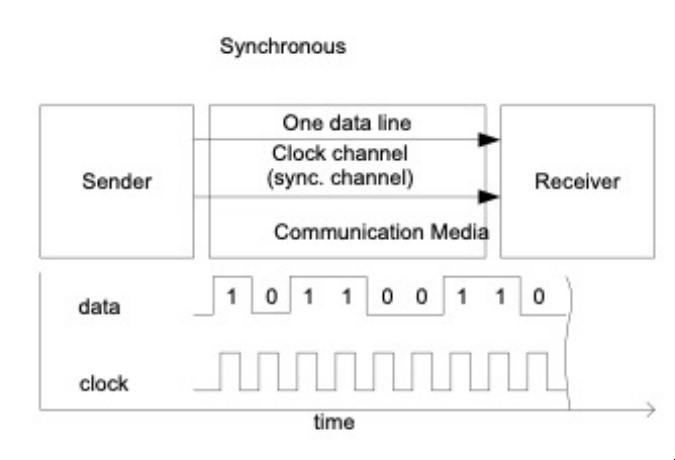
\includegraphics[width=0.6\textwidth]{serialsynch.png}
\end{center}

In the most common protocol of \textbf{asynchronous serial transmissions}, data is sent in small packets of 10 or 11 bits, 
eight of which constitute message information. 
When the channel is idle, the signal voltage corresponds to a continuous logic \verb|1|. 
A data packet always begins with a logic \verb|0| (the start bit) to signal to the receiver that a transmission is starting. 
The start bit triggers an internal timer in the receiver that generates the needed clock pulses. 
Following the start bit, eight bits of message data are sent bit by bit at the agreed upon baud rate. 
The packet is concluded with a parity bit \& stop bit. 
The packet length is short in asynchronous systems to minimise the risk that the local oscillators in the receiver \& transmitter will drift apart. 
When high-quality crystal oscillators are used, synchronisation can be guaranteed over an 11-bit period. 
Every time a new packet is sent, the start bit rests the Synchronisation, so the pause between packets can be arbitrarily long. 
\begin{itemize} 
    \item   Packet length is short (to minimise local oscillators drift). 
    \item   Examples: RS232 
\end{itemize}

\begin{center}
    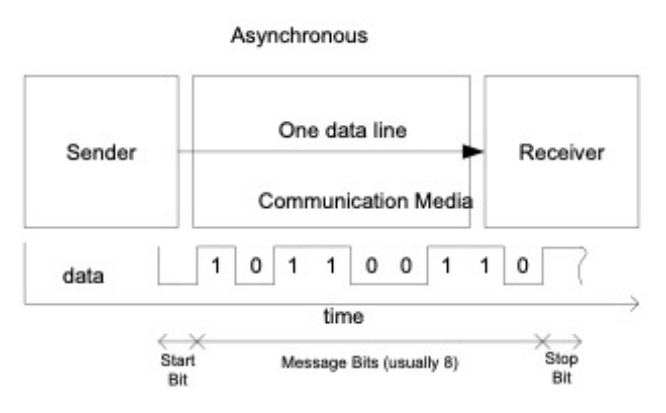
\includegraphics[width=0.6\textwidth]{serialasynch.png}
\end{center}

\subsection{Noise \& Distortion}
Long conductors act like receiving antennae for electrical noise radiated by motors, switches, \& other electrical circuits. 
Electrical signals get distorted when passing through metallic conductors due to limitations of bandwidth \& internal thermal noise of the transmission media. 


Because of the high switching rate \& relatively low signal strength found on buses within a computer (such as data, address, etc.), 
direct extension of the buses beyond the boundaries of the main circuit board or plug-in boards would pose serious problems. 
\begin{itemize}
    \item   Firstly, long runs of electrical conductors, either on printed circuit boards or through cables, act like receiving antennae 
            for electrical noise radiated by motors, switches, \& electronic circuits. 
    \item   A second problem involves the distortion of electrical signals as they pass through metallic conductors. 
            Signals that start at the source as clean, rectangular pulses may be received as rounded pulses with ringing at the 
            rising \& falling edges. 
\end{itemize}

\begin{center}
    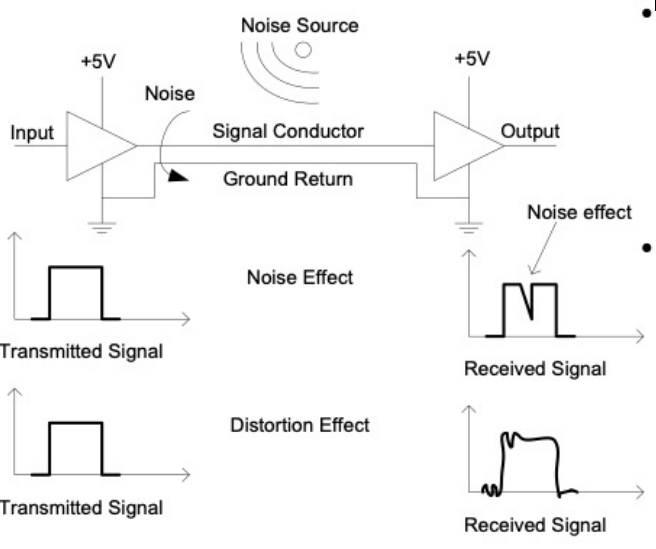
\includegraphics[width=0.6\textwidth]{noisendistortion.png}
\end{center}

\subsubsection{Noise Compensation}
Distortion effects are properties of transmission through metallic conductors, and become more pronounced as the conductor length 
increases. 
To compensate for distortion, signal power must be increased or the transmission rate decreased. 

Special amplifier circuits are designed for transmitting directly (un-modulated) digital signals through cables. 
For the relatively short distances between components on a printed circuit board or along a computer backplane, the amplifiers 
are in simple IC chips that operate from standard +5V power. 
The normal output voltage from the amplifier for logic \verb|1| is slightly higher than the minimum needed to pass the logic 
\verb|1| threshold. 
Correspondingly, for logic \verb|0|, it is slightly lower. 
The difference between the actual output voltage \& the threshold value is referred to as the \textbf{noise margin}, and 
represents the amount of noise voltage that can be added to the signal without creating an error. 

\begin{center}
    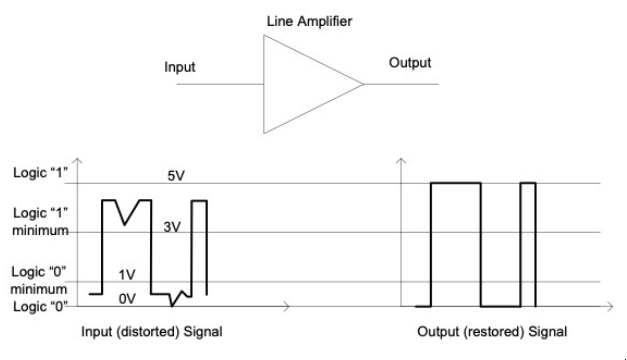
\includegraphics[width=0.6\textwidth]{noisecomp.png}
\end{center}

\subsubsection{Data Transfer over Long Distances} 
When relatively long distances are involved in reaching a peripheral device, driver circuits must be inserted after the bus 
interface unit to compensate of the electrical effects of long cables (noise \& distortion). 
This is the only change needed if a single peripheral is used. 

However, if many peripherals are connected, or if other computer stations are to be linked, a Local Area Network (LAN) is 
required, and it becomes necessary to drastically change both the electrical drivers \& the protocol to send messages through the 
cable. 
Because multi-conductor cable is expensive, bit-serial transmission is almost always used when the distance exceeds 10 meters. 

In either a simple extension cable or a LAN, a balanced electrical system is used for transmitting digital data through the channel. 
This type of system involves at least two wires per channel, neither of which is a ground. 
Note that a common ground return cannot be shared by multiple channels in the same cable as would be possible in an unbalanced system. 

\begin{center}
    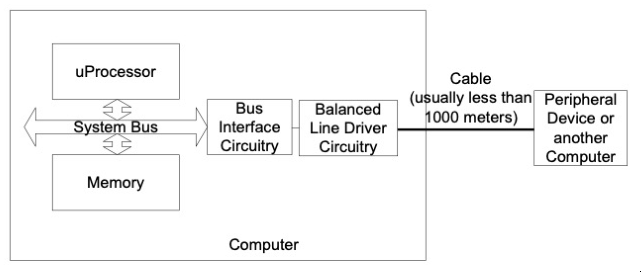
\includegraphics[width=0.6\textwidth]{dtold.png}
\end{center}

\subsubsection{Balanced Line Transmission}
The basic idea behind a \textbf{balanced line circuit} is that a digital signal is sent on \textit{two wires simultaneously},
one wire expressing a \textit{positive voltage image} of the signal, and the other a \textit{negative voltage image}.
When both wires reach the destination, the signals are subtracted by a \textbf{summing amplifier}, producing a signal swing of 
twice the value found on either incoming line. 
If the cable is exposed to radiated electrical noise, a small voltage o the same polarity is added to both wires in the cable. 
When the signals are subtracted by the summing amplifier, the noise cancels out, and the signal emerges from the cable without noise. 

\begin{center}
    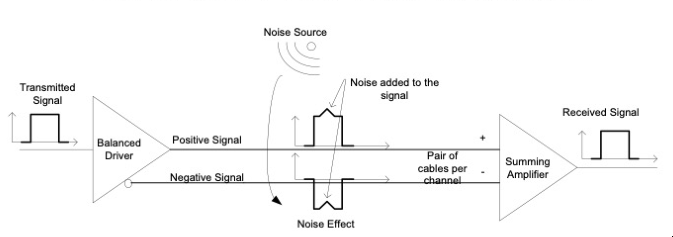
\includegraphics[width=0.8\textwidth]{ballinetrans.png}
\end{center}
\begin{itemize}
    \item   The signal is sent over \textbf{two} wires simultaneously. 
            \begin{itemize}
                \item   One wire is carrying the positive signal. 
                \item   One wire is carrying the negative (inverted) signal. 
            \end{itemize}
    \item   At the receiver, the signals are subtracted by a summing amplifier producing a stronger signal than any of the signals 
            swinging on the individual lines. 
    \item   When the signals are subtracted, any induced noise cancels. 
\end{itemize}

\subsection{Guided Transmission Data} 
\subsubsection{Twisted Pair} 
\textbf{Twisted Pair} consists of two insulated copper wires, typically about 1mm thick. 
The wires are twisted together in a \textit{helical} form. 
Twisting is done because two parallel wires constitute a fine antenna. 
When the wires are twisted, the waves radiated from different twists cancel each other out. 
The wires are usually bundled together \& encased in protective shields when coming from, say, a block of apartments to a phone 
company. 
If the wires were not twisted, the interference between the wires part of the same bundle would be significant.

Twisted pair wires can be used for the transmission of both digital \& analog signals. 
The bandwidth depends on the thickness of the wire \& the distance, but usually several Mbps can be easily achieved. 

Cat 2 UTP (16 MHz) was used until 1988 to wire telephone systems, but was later replaced by Cat 5 UTP and later variants 
(with more twists per centimeter, resulting in less cross-talk and better quality signals over longer distances), able to handle about 
100Mhz. 
Later categories include 6 \& 7, which are able to handle signals of 250MHz \& 600MHz, therefore having higher data rates 
over longer distances. 

\begin{center}
    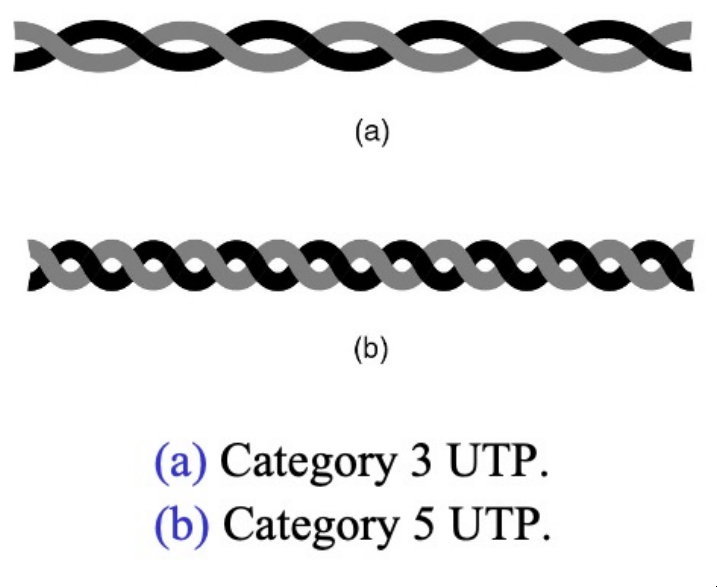
\includegraphics[width=0.5\textwidth]{twistedpair.png}
\end{center}

\subsubsection{Coaxial Cable}
\textbf{Coaxial Cables} are better shielded than twisted pair cables and can span over longer distances at higher speeds. 
50 Ohms (for digital transmission) \& 75 Ohms (for analog transmission) are available. 
Due to the construction \& the shielding process, the coax cables can have large bandwidth, up to 1GHz. 
Coaxial cables used to be largely utilised by phone companies for long distance lines, but have now been replaced with 
fibre optics. 

\begin{center}
    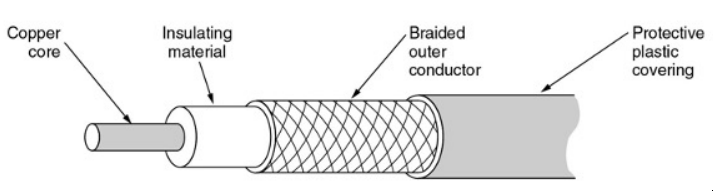
\includegraphics[width=0.5\textwidth]{coax.png}
\end{center}

\subsubsection{Fibre Optics}
The achievable bandwidth for optical fibre is in excess of 50Tbps (50,000 Gbps). 
However, the current practical signalling limit is 10Gbps, due not to the characteristics of the optical fiber, but by our 
inability to convert electrical signals into optical signals any faster. 

An \textbf{Optical Transmission System} has three components:
\begin{itemize}
    \item   The light source. 
    \item   The transmission medium. 
    \item   The detector.
\end{itemize} 

Conventionally, a pulse of light indicates a \verb|1| \& an absence of light indicates \verb|0|. 
The transmission medium is a thin optical fibre, and the detector generates an electrical pulse when light falls on it. 
By attaching the source of light at one end of an optical fibre, and the detector at the other end, we have a 
\textbf{unidirectional} data transmission system that accepts electrical signal, converts it into light, transmits it over 
the optical fibre, and is received by the detector and transformed back into electrical signal. 

The angle at which the light is injected into the optical fibre is very important. 
Because of refraction, the light can either escape the fibre, or be ``trapped'' inside it, with virtually no loss. 

\begin{center}
    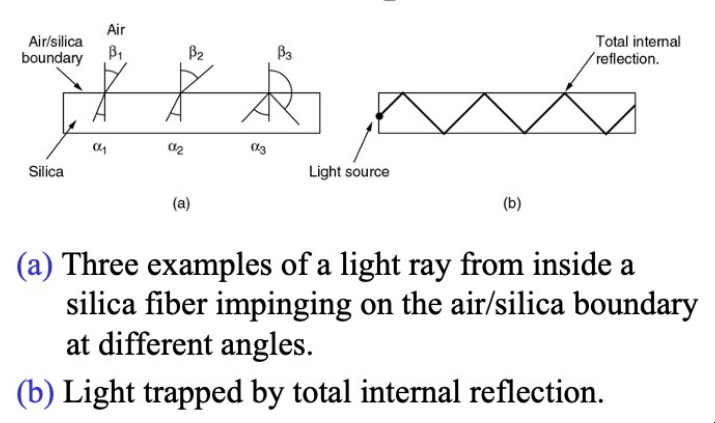
\includegraphics[width=0.5\textwidth]{fibopt.png}
\end{center}

In a \textbf{multimode fibre}, many different rays could bounce inside of the fibre, at different angles. 
In a \textbf{single mode fibre}, the diameter of the fibre is reduced to a few wavelengths of light, which causes the 
light to propagate only in straight lines. 
Single mode fibres are more expensive, and are used for transmission on very long distances. 
50Gbps for over 100Km are possible, without any amplification. 

\begin{center}
    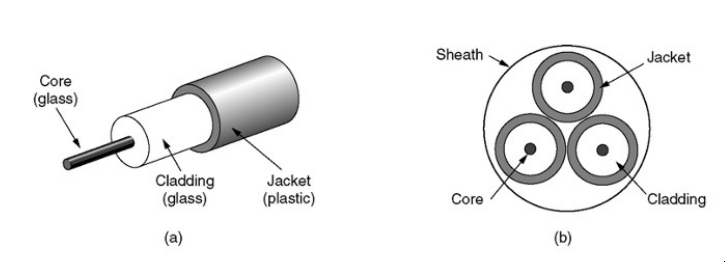
\includegraphics[width=0.8\textwidth]{p31.png}
\end{center}

For multimode fibres, the core is 50 microns. For single mode fibres, the diameter of the core is 8 to maximum 10 microns. 
Fibres can be connected in three ways: connectors, splicing, \& fusing.

\begin{center}
    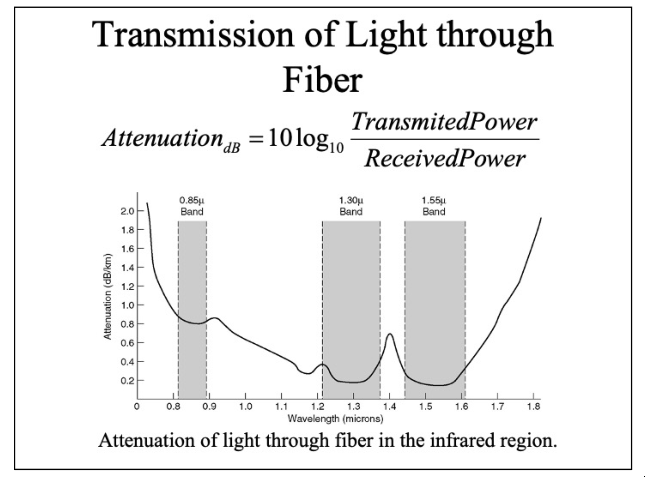
\includegraphics[width=0.6\textwidth]{translightfibre.png}
\end{center}

The attenuation of light through glass (the raw material used for optical fibre cables) depends on the wavelength of the 
light \& the physical properties of the glass. 
For example, an attenuation of 2 is given by $10 \text{log}_2 = 3\text{dB}$. 
Visible light is from 0.4 to 0.7 microns (400 to 700nm). 
Three wavelength bands are used for communication, centred on: 0.85 microns, 1.30 microns, \& 1.55 microns. 

As the ray of light travels down the fibre, \textbf{chromatic dispersion} (the process of spreading of the wavelength) is 
occurring. 
By making the pulses of a special shape, called \textbf{solitons}, nearly all the dispersion effects can be cancelled out. 

\begin{center}
    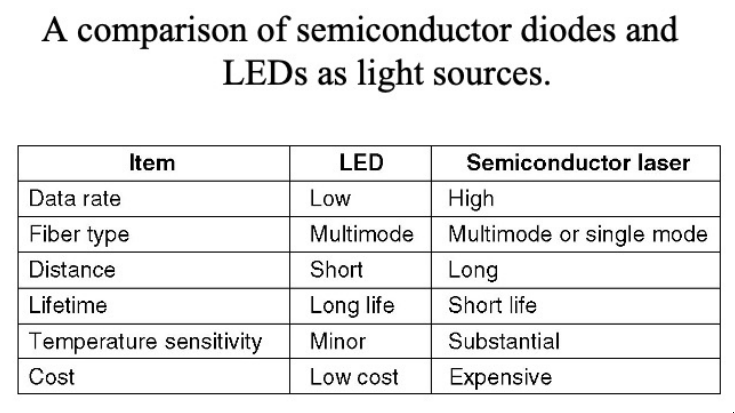
\includegraphics[width=0.6\textwidth]{compfibre.png}
\end{center}

Two types of light sources can be used: LED \& Semiconductor Lasers. 
The receiver is a \textbf{photodiode}, which gives an electrical pulse when struck by light. 
The response time is usually 1 nanosecond, which limits the data rates to about 1Gbps. 

\begin{center}
    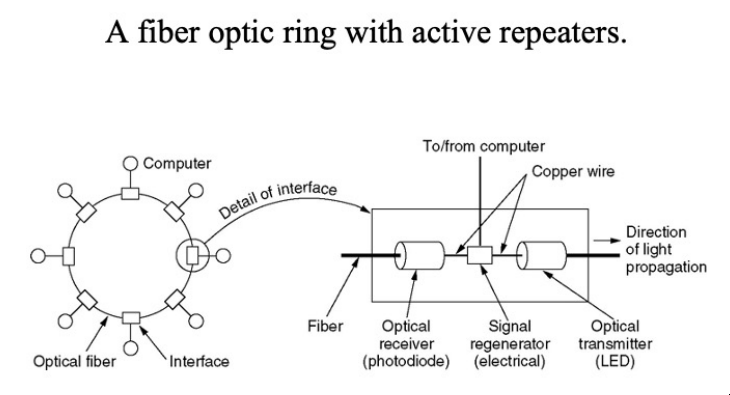
\includegraphics[width=0.7\textwidth]{fibpotnet.png}
\end{center}

A ring network is just a collection of point-to-point links. 
The interface on each computer passes the light pulse stream through to the next link and also serves as a T-junction to allow the 
computer to send \& accept messages. 
The interfaces could be \textbf{passive} (tapping an LED \& a photodiode on the fibre) or \textbf{active} (presented in the above figure). 
The passive interface loses signal, so therefore, the light cannot travel very far, and the size of the network is limited.
If an active repeater fails, the ring is broken and the network goes down. 

\subsection{Wireless Transmission} 
\subsubsection{The Electromagnetic Spectrum}
The number of oscillations per second of a wave is called its \textbf{frequency} ($f$), measured in Hertz.
The distance between two consecutive maxima (or minima) is called \textbf{wavelength} $\lambda$, measured in metres.
\textit{In vacuo}, all electromagnetic waves travel at the same speed, which is the speed of light $\sim3 \times 10^8$ m/s. 
In copper, all waves travel at about $\frac{2}{3}$ the speed of light.

The relation between the frequency \& wavelength of an electromagnetic wave (\textit{in vacuo}) is given by the relation:
$$ \lambda f = c $$

Since $c$ is a constant (the speed of light), if we know the frequency, then we can compute the wavelength, and vice-versa. 

\begin{center}
    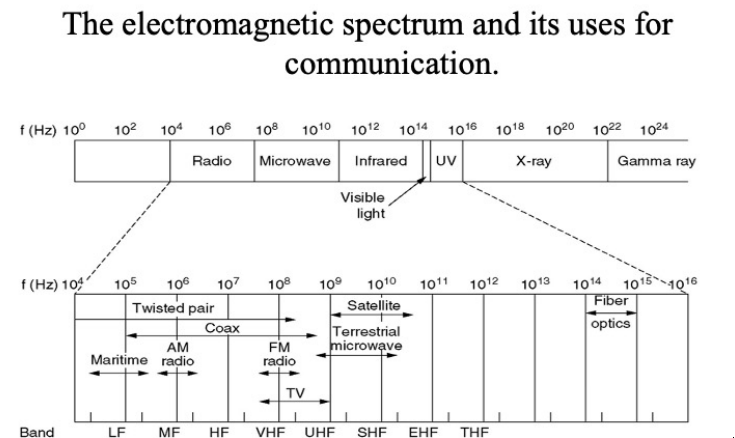
\includegraphics[width=0.7\textwidth]{electrospec.png}
\end{center}

Almost all transmissions use a narrow frequency band (with few exceptions - frequency hopping spread spectrum \& direct sequence spread 
spectrum). 
For the moment, we assume all transmission do use a narrow frequency band. 

\subsubsection{Radio Transmission}
\begin{center}
    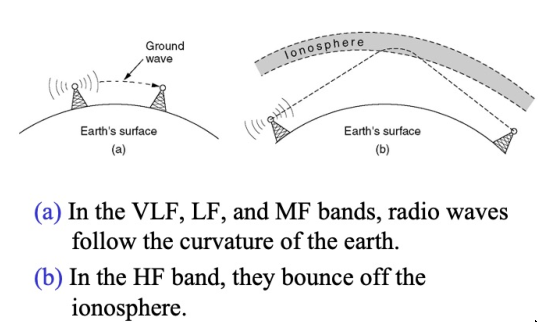
\includegraphics[width=0.6\textwidth]{radiotrans.png}
\end{center}

\subsubsection{Microwave Transmission}
Microwaves travel in straight lines above 1000MHz. 
If two points are too far apart, \textbf{repeaters} are needed between them. 
Microwaves can't pass through buildings, and if over 5GHz, the waves will be absorbed by water such as rain. 
Microwave transmission is widely used for long-distance communication, which has resulted in a shortage of available bandwidth. 

Microwaves have a \textbf{multipath fading} problem. 
Multipath fading refers to the fact that delayed waves may arrive out of phase with the direct wave and thus cancel the signal. 
Some operators keep their channels idle as spares to switch on when multipath fading wipes out some frequency band temporarily. 
Multipath fading is a phenomenon that is dependant on weather \& the operating frequency. 

\subsection{Politics of the Electromagnetic Spectrum}
Because radio is capable of travelling long distances, \textbf{interference} between users is a problem. 
For this reason, governments license the use of radio transmitters. 

The \textbf{Industrial, Scientific, and Medical} band (ISM) is different from country to country.

\begin{center}
    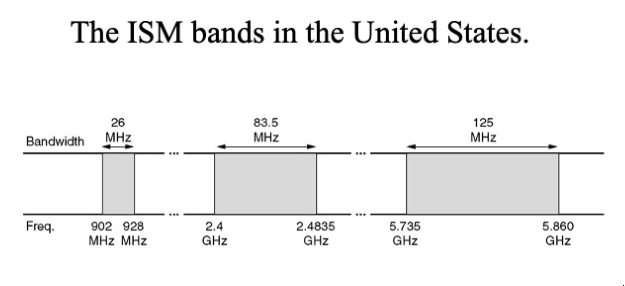
\includegraphics[width=0.6\textwidth]{ism.png}
\end{center}

\subsection{Infrared \& Millimeter Waves} 
Infrared \& millimeter waves are widely used for short range communications (i.e., used in remote controls). 
They are directional \& easy to build but don't pass through objects. 
However, this is also a plus, because it means no interference with similar systems sitting in the next room, no security issues, etc. 
No government license is needed to operate infrared systems. 

Infrared \& millimeter waves are also sometimes used in interconnecting some devices as well, i.e., mice to computers, mobile phones to other equipment, etc. 
The more we go from long wave radio towards visible light, the electromagnetic waves behave more \& more like light and less \& 
less like radio. 

\subsection{Communication Satellites} 
In its most simple form, a \textbf{communication satellite} can be seen as a big microwave repeater up in the sky. 
It contains several transponders, each of which listens to some portion of the spectrum, amplify the incoming signal, and then 
rebroadcast it to another frequency to avoid interference with the incoming signal. 
The downward beam can be \textit{broad} (covering a large area of Earth's surface) or can be \textit{narrow} (covering only a few hundred kilometers 
in diameter).

Issues with satellites:
\begin{itemize}
    \item   \textbf{Orbital Period -} The higher the satellite, the larger the orbital period. 
            (At an altitude of about 36,800km, the period is about 24 hours. At 384,000 km, the period is about 1 month). 
    \item   Presence of the \textbf{van Allen belts -} Layers of highly charged particles trapped by the Earth's magnetic field. 
            Any satellite flying inside of those belts would be quickly destroyed. 
\end{itemize}

\begin{center}
    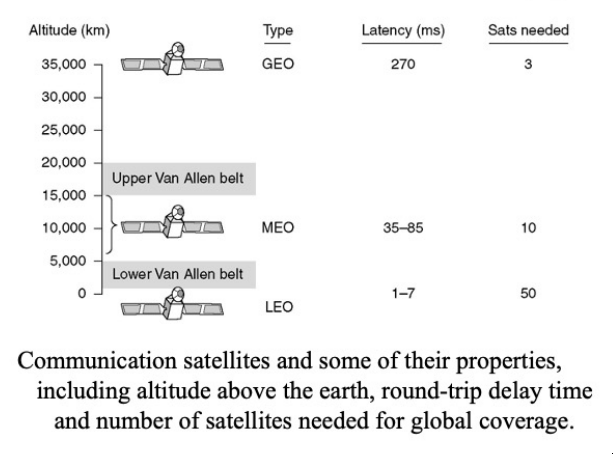
\includegraphics[width=0.6\textwidth]{comsat1.png}
\end{center}

\textbf{Geostationary Earth Orbit (GEO)} satellites sit at an altitude of about 35,800km in a circular equatorial orbit. 

\begin{center}
    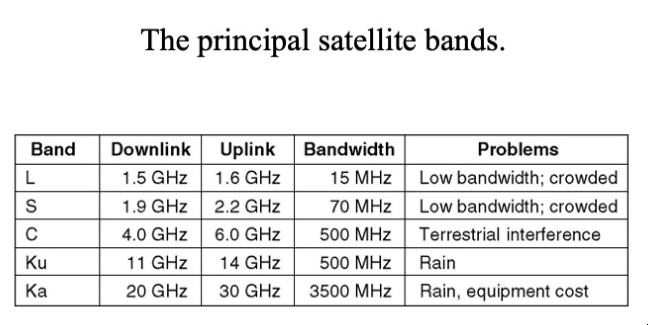
\includegraphics[width=0.6\textwidth]{comsat2.png}
\end{center}

\textbf{Very Small Aperture Terminals (VSATs)}  can be 1 metre in size or smaller, in contrast to the 10 meters required for 
GEO satellites communication. 

\begin{center}
    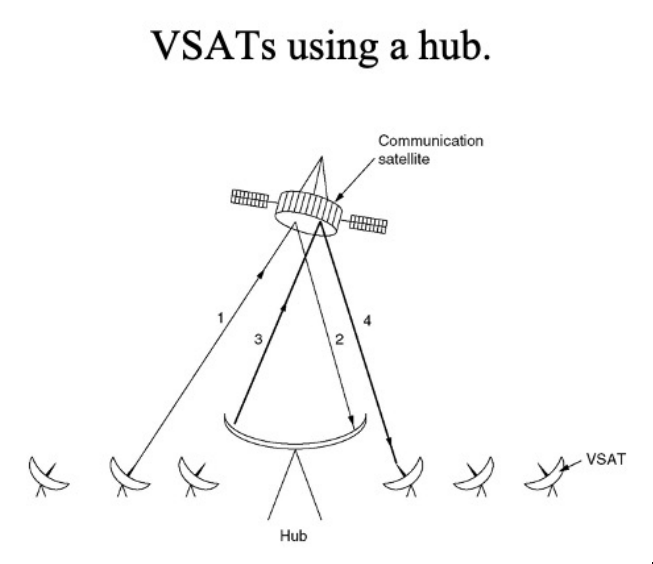
\includegraphics[width=0.6\textwidth]{vsathub.png}
\end{center}

\subsubsection{Middle Earth Orbit Satellites}
\textbf{Middle Earth Orbit (MEO)} satellites sit between the two van Allen belts. 
They must be tracked as they move through the sky. 
Less powerful transmitters are required to reach them. 
MEO satellites are not usually used for communication. 
One example of their use is \textbf{General Positioning System (GPS)} satellites. 
Currently, there are about 30 MEO satellites used the GPS system orbiting at about 18,000km.
GPS needs a minimum of 24 satellites to operate and the typical number of active GPS satellites is about 30. 
GPS receivers released since 2018 have much higher accuracy, pinpointing to within 30 centimeters. 

\subsubsection{Low Earth Orbit Satellites}
\textbf{Low Earth Orbit (LEO)} satellites sit below the van Allen belts.
Due to their motion, a large number of LEO satellites are required for full coverage. 
Because they are low orbit, the ground stations that communicate with them do not need much power, and the round trip is only 
a few milliseconds. 
Examples include Iridium and Starlink. 

\begin{center}
    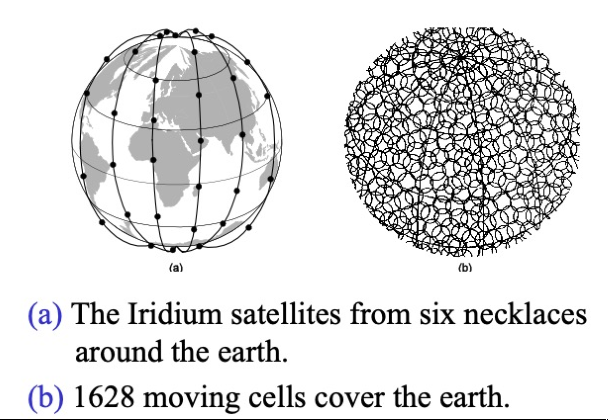
\includegraphics[width=0.6\textwidth]{iridium.png}
\end{center}

\subsection{Modems}
Due to attenuation (and other discussed problems), square waves (digital signal) cannot be used for long-distance transmission. 
Instead, AC signalling is used, with a continuous tone, around 1000 - 2000Hz, called a \textbf{sine wave carrier}. 
The amplitude, frequency, or phase of this AC signal can be \textbf{modulated} to transmit information.

\textbf{Modulation} is a technique by which analogue signals are used as carriers for digital signals. 
Many types of modulation are possible, including amplitude, frequency, \& phase modulation. 
\begin{itemize}
    \item   \textbf{Amplitude Modulation -} Two different amplitudes are used to represent \verb|1| or \verb|0|. 
    \item   \textbf{Frequency Modulation -} Two (or more) different tones are used. Also called Frequency Shift Keying. 
    \item   \textbf{Phase Modulation -} The carrier wave is shifted $0^\circ$ or $180^\circ$ at bit intervals to show a transition. 
            A better scheme is to use shifts of $45^\circ$, $135^\circ$, $225^\circ$, or $315^\circ$ to transmit two bits of information. 
\end{itemize}

\textbf{Modems} (\textbf{Mo}dulator/\textbf{Dem}odulator) are special devices which are connected to the computer system 
through techniques covered in Communication over Short Distances. 
Modems accept a serial stream of bits as input and produce a carrier modulated by one or more of the aforementioned methods. 
The modem is inserted between the digital computer and the analog telephone system.

\begin{center}
    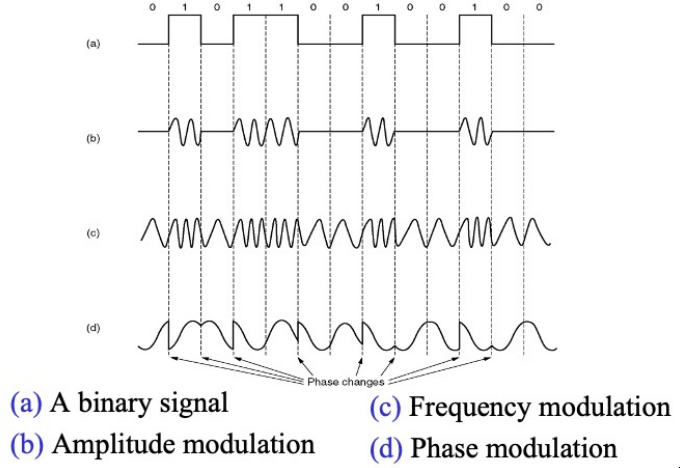
\includegraphics[width=0.6\textwidth]{modems1.png}
\end{center}

A good example of data communications over longer distances using copper wire is the use of the telephone network for one's 
home internet connection. 
Transmissions over such distances are not generally accomplished with a digital-wire link, unless you have fibre to the home, 
but rather with digitally-modulated analog carrier signals, as these are easier to transmit intact over a bandwidth-limited link 
to the ISP. 
This technique makes it possible to use existing phone lines for digital data, although at possibly reduced data rates 
compared to a direct digital link. 

Transmission of data from one's home over phone line requires that data signals be converted to \textbf{modulated carrier waves} 
by a \textbf{modem}.
One or more sine wave carriers are used, and, depending on the baud rate \& protocol, the modem will encode data by varying the 
frequency, phase, or amplitude of the carrier. 
The receiver's modem accepts the modulated sine wave \& extracts the digital data from it. 
Several modulation techniques are typically used in encoding digital data for transmission. 

A phone line has a band of 3,000Hz, so, by Nyquist theorem, there is no point in sampling the line at faster rates than 6,000 times per second. 
In practice, most modems sample at 2,400 times per second and focus on getting more bits per sample.
The number of samples per second is measured in \textbf{baud}. 
During one baud, one \textit{symbol} is sent.
One symbol can consist of one or more bits.
$n$ baud line transmits $n$ symbols per second. 
A 2400bps line transmits one symbol about every 416.667 microseconds. 
If the symbol consists of 2 bits per symbol, then the bit rate is 4800 bits per second.
    
\begin{itemize}
    \item   The \textbf{bandwidth} of a medium is the range of frequencies that pass through with minimum attenuation. 
            It is a \textit{physical property} of the medium, 0 to some maximum frequency, measured in Hertz.
    \item   The \textbf{baud rate} is the number of samples made per second. 
            One symbol is sent out per sample, thus the baud rate \& the symbol rate are the same.
    \item   The \textbf{bit rate} is the amount of information sent over the channel. 
            It is equal to the number of symbols per second times the number of bits per symbol.
\end{itemize}

\begin{center}
    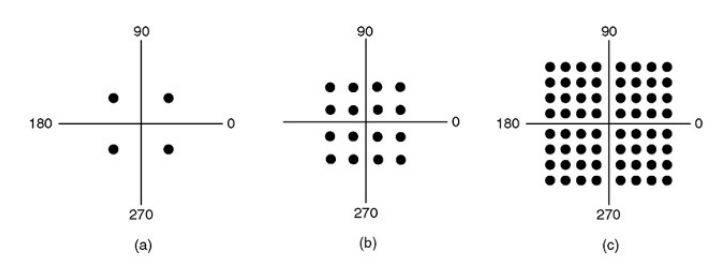
\includegraphics[width=0.6\textwidth]{moreaboutmodems.png}
\end{center}
The above diagrams are called \textbf{constellation diagrams}. 
Each constellation diagram shows the legal combinations of amplitude \& phase. 
Each modem uses its own constellation diagram and can talk only with modems that implement the same constellation diagram.

In \textbf{Quadrature Phase Shift Keying (QPSK)} four phases are used. 
In \textbf{Quadrature Amplitude Modulation 16 (QAM-16)}, four amplitudes \& four phases are used to form a total of \textbf{16} 
possible combinations. 
In other words, a symbol can encode 4 bits, 9600 bits per second over a 2400 baud line.
In \textbf{Quadrature Amplitude Modulation 64 (QAM-64)}, there are a total of 64 possible combinations.
In other words, a symbol can encode 6 bits.
Higher order QAMs are also used. 

\begin{center}
    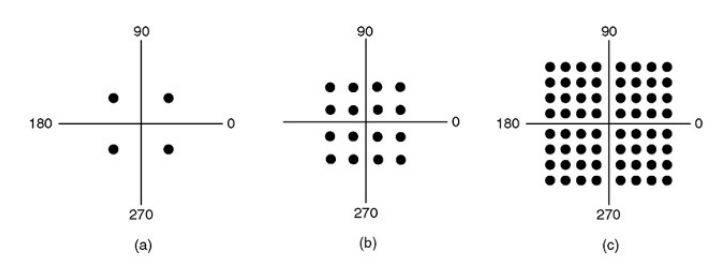
\includegraphics[width=0.6\textwidth]{moreaboutmodems.png}
\end{center}

With many points in the constellation diagram, even a small amount of noise would result in transmission errors.
\textbf{Trellis Coded Modulation (TCM)} is used, where besides the data, a symbol also contains \textbf{parity checking}. 

Modems are \textbf{bidirectional} devices, by using different frequencies for different directions. 
Bidirectional simultaneous connections are called \textbf{full duplex connections}.

\subsection{Digital Subscriber Lines} 
Services with more bandwidth than standard telephone services are called \textbf{broadband}, although the term is more 
marketing than technical. 

\textbf{Digital Subscriber Line (DSL)} services started to be offered by phone companies, to be competitive on the broadband 
services market (TV \& satellite companies were already offering broadband services). 

The reason why modems are so slow is that phone lines were invented to carry human voice, not data. 
Therefore, frequencies below 300Hz and above 3100Hz were artificially filtered out. 
Cutoff filters were added on the local loops to filter out frequencies other than voice. 
The cutoff is not sharp, so the bandwidth is usually quoted to be 4000Hz even though the distance between the 3dB points is 
3100Hz. 
Thus, data is restricted to this narrow band. 

The trick that made DSL (or \textbf{Asymmetric DSL (ADSL)}) work is that when a customer subscribes to it, the incoming 
line is connected to a different kind of switch in the end office that doesn't have this voice filter installed, thus 
making the entire capacity of the loop available. 

The capacity of the local loop depends on the length \& thickness of the cable, and a plot of it is presented below. 
Therefore, the ADSL services are limited to customers that are within a certain radius from the end office (phone 
company switch). 

\begin{center}
    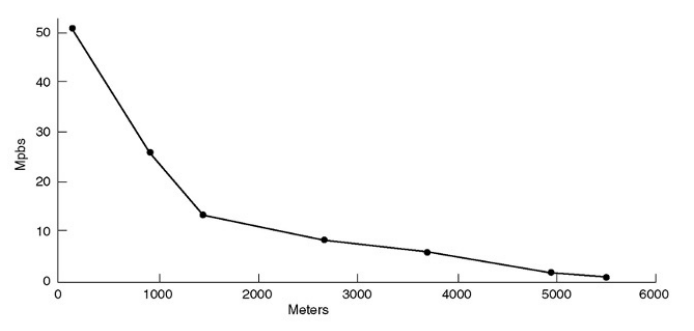
\includegraphics[width=0.8\textwidth]{dsl.png}
\end{center}

The available spectrum of the local loop (which is 1.1MHz for a decent service) is divided into 256 channels of 4312.5Hz each. 
Channel 0 is used for POTS (Plain Old Telephone Service). 
Channels 1 to 5 are not used, to make sure that there is enough guard between voice \& data. 
The remaining 250 channels are used for data \& stream control (one is used for upstream control \& one is used for 
downstream control). 
It is up to the provider how many channels will be used for upstream \& downstream. 
A 50-50 mix for upstream \& downstream is possible, but usually providers allocate more for downstream than for upstream, 
usually 80\% downstream, 20\% upstream, as most of the users are using the line for Internet, and thus pull pages down 
onto their system. 
This is why DSL turned into ADSL. 
A common split is 32 channels for upstream, and the rest for downstream. 

Within each channel, a modulation schema similar to V.34 is used, although the sampling rate is 4000 baud instead of 2400. 
The line quality in each channel is constantly monitored, and the data rate is adjusted continuously as needed, so 
different channels may have different data rates. 
The data is sent with QAM modulation, with a maximum of 15 bits per symbol. 
With 224 downstream channels, the downstream data bit rate is about 13.4Mbps. 
In practice, the signal to noise ratio is never good enough to achieve this bit rate, but 8Mbps is possible on short local 
loops, and the ADSL standard goes this far. 

\begin{center}
    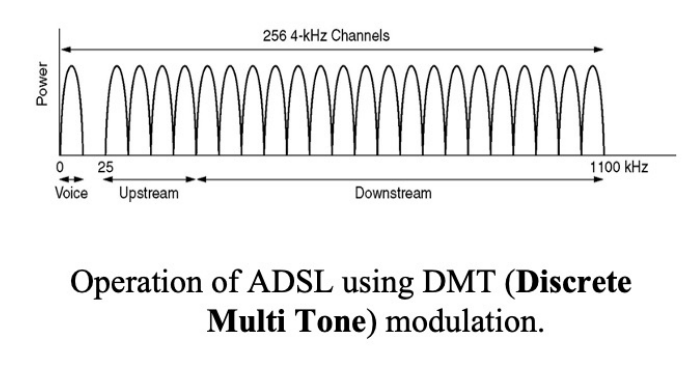
\includegraphics[width=0.8\textwidth]{dsl2.png}
\end{center}

A telephone company technician must install a \textbf{Network Interface Device (NID)} in the customer's house. 
Close to or combined with the NID, a \textbf{splitter} is installed, which is an analog filter which separates the phone signal 
(0 to 4000Hz) from the data signal (over 26kHz). 

The ADSL modem is actually a signal processor that acts as 250 QAM modems, operating in parallel at different frequencies 
available for each channel. 
Usually, the connection between the modem \& the computer is Ethernet-based. 

At the end office, a special \textbf{Digital Subscriber Line Access Multiplexer (DSLAM)} receives the data over 26kHz 
(separated by the splitter) and recovers the bit stream from the data (same function as the ADSL modem at the customer 
end). 
The low frequency signal (POTS signal), is sent to a conventional switch. 

\subsection{Trunks \& Data Multiplexing} 
High bandwidth \textbf{trunks} are available between switching offices. 
The data collected from end loops needs to be multiplexed over those high-bandwidth trunks. 
There are two main categories for data: \textbf{FDM} \& \textbf{TDM}. 
\begin{itemize}
    \item   In \textbf{Frequency Division Multiplexing (FDM)}, the frequency spectrum is divided into frequency bands, 
            with each user having exclusive possession of some band. 
    \item   In \textbf{Time Division Multiplexing (TDM)}, the users take turns (in a round robin fashion), each one 
            periodically getting the entire available bandwidth for a short period of time. 
\end{itemize}

\subsubsection{Frequency Division Multiplexing}
The below diagram presents how voice-grade telephone channels are multiplexed using FDM. 
When many channels are multiplexed together, 4kHz bandwidth is allocated to each channel to keep them separated. 
First, each channel is raised in frequency, each by a different amount. 
Then, they can be combined, because no channel will occupy the same portion of the spectrum/ 

FDM schemata are, to some degree, standardised. 
A widespread standard is twelve 4kHz voice channels multiplexed into sixty 108kHz baud.
This is called a \textbf{group}. 
Five groups can be multiplexed into a \textbf{supergroup}. 
Five supergroups can be multiplexed into a \textbf{mastergroup}. 

\begin{center}
    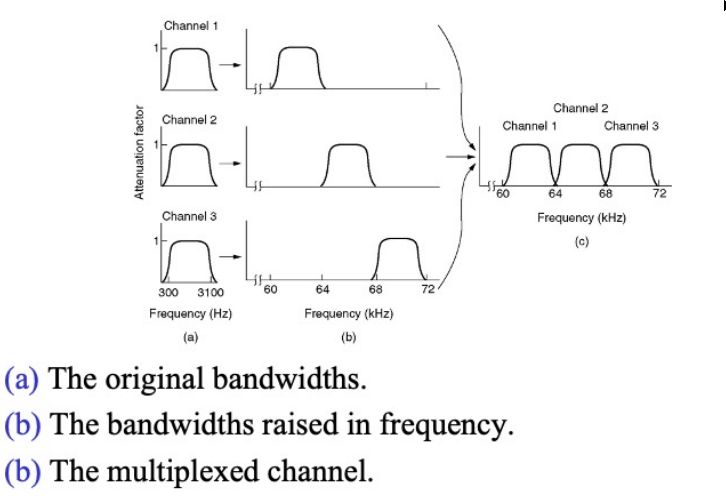
\includegraphics[width=0.8\textwidth]{fdm.png}
\end{center}

\textbf{Wavelength Division Multiplexing (DWM)} is a variation of FDM at very high frequencies, used primarily over 
optical fiber trunks. 
Systems with 96 channels of 10Gbps each are available in production. 
960Gbps is enough to send approximately 30 full movies per second.

\begin{center}
    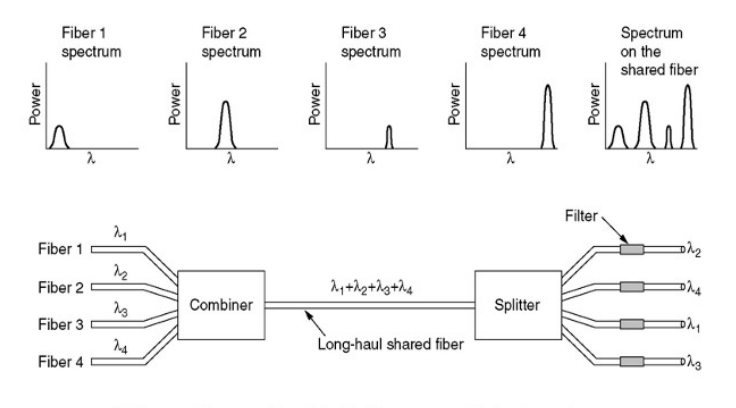
\includegraphics[width=0.8\textwidth]{wdm.png}
\end{center}

\subsubsection{Time Division Multiplexing} 
\textbf{Time Division Multiplexing} is how multiple analog telephone channels are digitised \& combined onto a single 
outgoing digital trunk. 
The analog data is digitised in the end office by a device called a \textbf{codec}. 
The codec makes 8000 samples per second (125 $\mu$s per sample, is, according to Nyquist's theorem, enough to sample at 
twice the bandwidth of the signal to capture all the information carried by the signal) and measures the amplitude of each 
sample with a precision of 8 bits. 
This process is called \textbf{Pulse Code Modulation (PCM)}, and forms the heart of the modern telephone service. 
As a consequence, all time intervals within a phone system are multiples of 125$\mu$s.

Incompatible schemata are in use in the US \& Europe; Japan \& the US use the T1 carrier (presented below), while the E1 
carrier is used in the EU. 

\begin{center}
    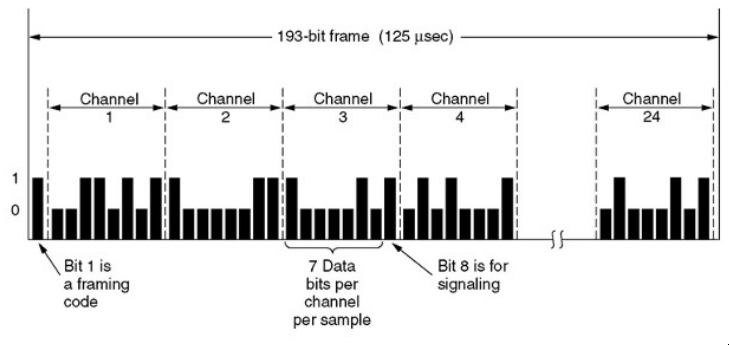
\includegraphics[width=0.8\textwidth]{tdm.png}
\end{center}

Each T1 frame accommodates 24 channels (each sampled 8000 times per second, 7 bits per sample), giving a gross data rate of 
1.544Mbps. 
An extra bit is used for framing control. 
This bit changes value from \verb|0| to \verb|1|, and from \verb|1| to \verb|0| every frame. 
The changing patter is \verb|01010101|\dots and is used by the receiver to ensure that it is not loosing synchronisation. 
Analog customers cannot generate this wave, as it corresponds to a sine wave at 4000Hz and this frequency is not present in 
analog voice channels.

E1 has 32 channels, with 8 bits per channel packed into the basic 124$\mu$s frame. 
This yields to a gross data rate of 2.048Mbps. 

\begin{center}
    \includegraphics[width=0.7\textwidth]{tdm2.png}
\end{center}

Once the voice channel has been digitised, it is tempting to use statistical techniques to obtain fewer bits per sample, thus 
requiring lower bandwidth to carry the voice information. 
All the compaction methods are based on the fact that the analog voice signal is changing relatively \textit{slowly} in 
comparison to the sampling frequency, so much so that that the information in the 7\textsuperscript{th} \& 8\textsuperscript{th}
bits is redundant. 

\textbf{Differential Pulse Control Modulation (DPCM)} is based on producing as output the difference between the current value 
and the previous one. 
Since jumps of $\pm 16$ in a scale from - to 128 are unlikely, just 5 bits are enough to represent the audio signal. 
If the signal does occasionally jump sharply, then a few samples are required to catch up with the new value. 
For human speech, this kind of error can be ignored. 

\textbf{Delta Modulation} is a variation of DPCM that requires the current value to differ by only $\pm1$ from the previous 
value. 
Under those conditions, just one bit can be sent to indicate if the next value is over or below the previous value. 

\begin{center}
    \includegraphics[width=0.7\textwidth]{tdm3.png}
\end{center}

\subsubsection{Cable Television} 
\begin{center}
    \includegraphics[width=0.7\textwidth]{communityantennatelevision.png}
\end{center}

\begin{center}
    \includegraphics[width=0.7\textwidth]{internetovercable.png}
\end{center}

\begin{center}
    \includegraphics[width=0.7\textwidth]{internetovercable2.png}
\end{center}

\begin{center}
    \includegraphics[width=0.6\textwidth]{spectrumallocation.png}
\end{center}

\begin{center}
    \includegraphics[width=0.6\textwidth]{cablemodems.png}
\end{center}

\section{Medium Access Control (MAC) Sublayer}
\subsection{The Channel Allocation Problem} 
In broadcast networks, the key issue is how to determine who gets to use the channel when there is competition for it.

\subsection{Multiple Access Protocols} 
\subsubsection{CSMA Protocols} 
\textbf{Carrier Sense Multiple Access (CSMA)} protocols are protocols in which stations listen for a carrier (i.e., transmission) 
and act accordingly. 
Networks based on these protocols can achieve better channel utilisation that $\frac{1}{2}$. 

CSMA Protocols include:
\begin{itemize}
    \item   1 Persistent CSMA. 
    \item   Non-Persistent CSMA. 
    \item   p-Persistent CSMA. 
    \item   CSMA CD. 
\end{itemize}

\textbf{1 Persistent CSMA}:
\begin{itemize}
    \item   When a station has data to send, it first listens to the channel. 
    \item   If the channel is busy, the station waits until the channel is free. 
            When it detects an idle channel, it transmits the frame. 
    \item   If collision occurs, it will wait a random amount of time and then start again. 
    \item   The protocol is called \textbf{1 Persistent} because the station sends with probability 
            of 1 when it finds the channel idle, meaning that it is continuously listening. 
    \item   The propagation delay has an important effect ton the performance of the protocol. 
            There is a small chance that just after a station begins sending, another station will 
            sense the channel is idle (before the signal from the first station reaches it). 
            The longer the propagation delay, the more important this effect becomes, and the worse 
            the performance of the protocol.
    \item   Even if the propagation delay is zero, there will still be collisions. 
            Imagine that two stations wanted to transmit data at the same time, but a third 
            station is busy transmitting.
            Both stations will wait until the third has finished transmitting, sense the idle channel, 
            \& begin sending.
\end{itemize} 

\textbf{Non-Persistent CSMA}:
\begin{itemize}
    \item   A station senses the channel before sending. 
            If there is no activity, it sends its frame. 
    \item   If the channel is busy, then instead of continuing to sense the channel until it becomes 
            idle, it simply retries at a later time by waiting a random period of time \& repeating the algorithm.
    \item   With this algorithm, fewer collisions will happen; thus better channel utilisation, at 
            the cost of longer delays than 1 Persistent CSMA algorithm
\end{itemize}

\begin{center}
    \includegraphics[width=0.7\textwidth]{persistentandnonpersistentcsma.png}
\end{center}

\textbf{p-Persistent CSMA}:
\begin{itemize}
    \item   Applies to \textit{slotted channels}. 
    \item   When a station becomes ready to send, it senses the channel. 
            If the channel is idle, then the station will transmit with a probability of $p$. 
            With a probability of $q$, it defers the next slot. 
    \item   If the next slot is also idle, it transmits or defers again with probabilities of $p$ \& $q$. 
    \item   This process is repeated until the frame either gets transmitted or another station begins 
            transmission. 
\end{itemize}

\textbf{CSMA with Collision Detection}:
\begin{itemize}
    \item   An improvement over CSMA protocols is for a station to abort its transmission when it sense a 
            collision. 
    \item   If two stations sense the channel idle \& begin transmission at the same time, they will both 
            detect the collision immediately. 
            There is no point in continuing to send their frames, since they will be garbled. 
    \item   Rather than finishing the transmission, they will stop as soon as the collision is detected, 
            saving time \& bandwidth.
    \item   This protocol is widely used. In particular, it is the basis for Ethernet LAN.
\end{itemize}

\begin{center}
    \includegraphics[width=0.7\textwidth]{csmawithcd.png}
\end{center}

\begin{itemize}
    \item   At the point marked $t_0$, a station has finished transmitting its frame. 
            Any other station that has a frame to send may now attempt to do so. 
            If two or more stations decide to transmit simultaneously, there will be a collision. 
            Collisions can be detected by looking at the power of the line or at the \textbf{pulse width} of 
            the received signal \& comparing it with the transmitted signal.
    \item   After a station detects a collision, it aborts its transmission, and waits a random period 
            of time before trying again. 
            Therefore, the CSMA/CD will consist of alternating contention \& transmission periods, with 
            idle periods occurring when all stations are quiet.
    \item   The minimum time to detect a collision is two times the time it takes the signal to propagate 
            from one station to another. 
            In worst-case scenarios, the two stations can be at the ends of the cable - Therefore, the 
            minimum time to detect a collision is the round-trip propagation delay for the whole cable 
            segment. 
    \item   The sending station has to monitor the channel for collision during transmission. 
            Therefore, CSMA/CD is a \textbf{half-duplex system}.
    \item   It is important to realise that the collision detecting is an analog process. 
            The station's hardware must listen to the cable while it is transmitting. 
            If what it reads back is different to what it sends, then a collision must have occurred. 
            The implication is that the signal encoding must allow collisions to be detected - i.e., 
            a collision of two 0V signals will never be detected. 
            For this reason, a special encoding is used.
\end{itemize}

\subsubsection{Collision-Free Protocols}
Collisions have an adverse effect on the system performance, especially if the cable is long \& the 
frames are short. 

The \textbf{collision-free protocols} solve the contention for the transmission channel without any 
collisions at all. 

$N$ stations are assumed to be connected to the same transmission channel.

Collision-free protocols include:
\begin{itemize}
    \item   Bit-Map protocol. 
    \item   Binary Countdown.
\end{itemize}

\begin{center}
    \includegraphics[width=0.7\textwidth]{bitmap.png}
\end{center}
\begin{itemize}
    \item   Each contention period consists of exactly $N$ slots. 
            If station 0 has a frame to send, then it transmits a slot during the 0\textsuperscript{th} 
            contention slot. 
            No other station is allowed to transmit during this slot. 
            Regardless of what station 0 does, station 1 gets the opportunity to transmit a \verb|1| bit during 
            contention slot 1, but only if it has a queued frame.
    \item   After all $N$ slots have passed, each station has complete knowledge of which stations wish to transmit. 
            At that point, they begin transmitting in numerical order. 
            Since everyone agrees who goes next, there are no collisions.
    \item   Protocols like this are called \textbf{reservation protocols}.
\end{itemize}

\begin{center}
    \includegraphics[width=0.7\textwidth]{binarycountdown.png}
\end{center}
\begin{itemize}
    \item   A problem with bitmap protocols is that the overhead per station is fixed (on bit), therefore 
            it does not scale well with a large number of stations. 
    \item   In the \textbf{binary countdown protocol}, all stations have the same address length.
            If a station wants to use the channel, the station broadcasts its address as a binary string, starting 
            with the high order bit.
            The bits in each address position from each station are \verb|OR|ed together. 
            This is called \textbf{binary countdown}.
            All the stations will see the result of the \verb|OR| operation simultaneously. 
            For example, if a station that placed a \verb|0| on the channel sees a \verb|1|, then it will stop trying.
            A higher-priority station wants to transmit, so it must stop trying.
    \item   In other words, as soon as a station has seen that a high-order bit in its address with value \verb|0| has 
            been overwritten with a \verb|1|, it gives up.
    \item   Imagine the stations \verb|0010|, \verb|0100|, \verb|1001|, \& \verb|1010| are all trying to get the 
            channel.
            The station with the address \verb|1010| gets the channel, as this protocol gives priority to the stations with 
            higher addresses.
\end{itemize}

\subsubsection{Wireless LAN Protocols}
\begin{center}
    \includegraphics[width=0.7\textwidth]{wirelesslanprotocolsp14.png}
\end{center}
\begin{itemize}
    \item   It is important to note that in a wireless LAN system, not all stations are within the range of the others. 
            Due to this, the \textbf{hidden station problem} can occur - When station $A$ transmits, station $C$ can't 
            sense it and may transmit too, resulting in the frame from station $A$ to station $B$ becoming garbled. 
            For this reason, a simple CSMA approach will not work for wireless LANs.
    \item   The reverse problem, called the \textbf{exposed station problem} can also occur. 
            If $B$ transmits to $A$, and $C$ senses it, $C$ may falsely conclude that it may not send to $D$, when in fact 
            such a transmission would only cause bad reception in regions between $B$ \& $C$.
    \item   Before starting a transmission, a station wants to know if there is activity around the receiver.
\end{itemize}

\begin{center}
    \includegraphics[width=0.7\textwidth]{macaprotocol.png}
\end{center}
\begin{itemize}
    \item   In \textbf{MACA (Multiple Access with Collision Avoidance)}, the sender stimulates the receiver to output 
            a short packet, so the stations around it will hear it and understand to avoid transmission during the 
            upcoming (large) data frame.
    \item   In the above graphic, station $A$ wants to send data to station $B$. 
            A short exchange of packets \textbf{RTS} (Request To Send) \& \textbf{CTS} (Clear To Send) takes place.
            The RTS frame (short frame, < 30 bytes) contains the length of the data frame that is about to be transferred.
            This data is copied into the CTS frame by the receiver.
            When $A$ receives the CTS frame, it begins the transmission of the data frame.
\end{itemize}

\subsection{Ethernet}
\subsubsection{Historic Ethernet Cabling}
\begin{center}
    \includegraphics[width=0.7\textwidth]{threekindsofethernetcabling.png}
\end{center}
\begin{itemize}
    \item   In 10Base5, the transceiver \& the interface board are separated. 
            The interface board goes inside the computer, while the transceiver goes on the cable (close to the vampire tap). 
            The transceiver contains the electronics that handle the collision detection.
    \item   In 10Base2, the connection to the cable is just a passive BNCT junction. 
            The transceiver electronics are situated on the controller board inside the PC.
    \item   In 10BaseT, there is no shared cable at all, just the hub. 
            Each station is connected to the hub using a dedicated, non-shared cable.
\end{itemize}

\subsubsection{The Ethernet MAC Sublayer Protocol}
\begin{center}
    \includegraphics[width=0.7\textwidth]{ethernetmacsublayerprotocol.png}
\end{center}

There are two variants of Ethernet, but the differences are minor and they are interoperable:
\begin{itemize}
    \item The initial one: DIX (Initiated by Xerox, Intel, \& DEC). 
    \item The IEEE 802.3 standard.
\end{itemize}

Each frame starts with a \textbf{Preamble} of 8 bytes in DIX or 7 bytes in IEEE 802.3, each containing the bit pattern
\verb|10101010|\dots
The Manchester encoding on this pattern produces a 10MHz square wave for 6.4$\mu$s to allow the receiver's clock 
to synchronise with the sender.
The clock will stay in sync for the rest of the frame, using the transitions in the middle of the bit boundaries 
for adjustment.
The IEEE frame also contains a \textbf{Start Frame Delimiter (SFD)} which signifies that the next byte begins the 
Destination MAC Address field.

In Ethernet addresses, the high order bit distinguishes between normal addresses \& group addresses (\verb|1| for 
group, \verb|0| for normal). 
This allows multiple stations to listen to one address so that when a frame is sent to a group address, all the 
stations in the group receive it.
The second high order bit distinguishes between local \& global addresses (\verb|1| for local, \verb|0| for global).  
All \verb|1|s (\verb|ff:ff:ff:ff:ff:ff|) is reserved for the broadcast address.

The \textbf{type} field in DIX tells the receiver what to do with the frame. 
Multiple network protocols could be supported, so this field is unique for each network protocol. 
The type field is used to dispatch the incoming frames. 
IEEE 802.3 changed the type field to the \textbf{length} field - the type is handled as part off the data itself, 
in a small header.
The length field contains the length in bytes of the data, up to 1500 bytes.
There is also a minimum length, related to the collision detection.
The minimum Ethernet frame length is 64 bytes (without the preamble), and if the data portion is less than 46 bytes
(64 - (headers + checksum)), then the PAD field is used to fill the frame to the minimum size.

The \textbf{checksum} is a 32-bit hash code of the data, computed with the CRC algorithm presented in the Data 
Link Layer, and has a 32 order generator polynomial.
This just does error detection, no forward error correction.

\begin{center}
    \includegraphics[width=0.7\textwidth]{ethernetmacsublayerprotocol2.png}
\end{center}

The strongest reason why there is a minimum length for the Ethernet frame is to allow the CSMA/CD protocol to 
work properly. 
The collisions should be detected by the transmitting station, or preventing a transmitting station to finish the 
transmission of a frame until the first bit reached the far end of the cable, where it may collide with another 
frame.

If we have a collision at time $\tau$, the station $B$ (that detected the collision first), issues a 48-bit noise burst 
(known as a \textbf{jam signal}) to warn the other stations.
At about $2\tau$ time, the sender (station $A$) will see the noise burst and abort its transmission too. 
$A$ will wait a random amount of time until it tries again.

For a 2500 meter LAN with 4 repeaters, the round trip time (the propagation time for a signal to travel from one 
end of the LAN to the other end of the LAN and back) is about 50$\mu$s. 
This is equivalent to about 500 \textit{bit times} (one bit time for a 10Mbps network is 100ns).
Therefore, a station should be in transmit mode for at least 500 bit times, which gives us the minimum Ethernet 
frame of about 500 bits. 
The standard's choice was 512 bits or 64 bytes minimum per frame.

Frames with fewer than 64 bytes will be padded out to 64 bytes.
As the network speed goes up, the minimum frame length does too.

\subsubsection{The Binary Exponential Back-Off Algorithm}
After a collision, the time is divided into discrete slots (equal to the worst-case round-trip propagation time, 
which is 521 bits time or 52.2$\mu$s).
After the first collision, each station waits 0 or 1 time slots before it tries again. 
If two stations collide, and they pick the same number, they will collide again.

After a second collision, each station randomly waits 0, 1, 2, or 3 time slots.
After a third collision, the next number of time slots to be picked is between 0 and $2^3 -1 $ and that number of 
slots is skipped.
After 10 collisions have been reached, the number interval is frozen at 0-1023.

After 16 collisions, the station gives up sending the frame and reports the failure. 
Further recovery is up to the higher layers.

\subsubsection{Modern Switched Ethernet} 
\begin{center}
    \includegraphics[width=0.7\textwidth]{modernswitchedethernet.png}
\end{center}

If more stations are added onto an Ethernet LAN, the traffic will go up. 
Eventually, the LAN will become saturated.

Switches are typically devices that have 4 to 32 plug-in cars, each with 1 to 8 Ethernet connectors (RJ45)/ 
When a station wants to send an Ethernet frame, the plug-in card getting the frame will check to see if the 
destination address is one of the cards connected onto one of its ports.
If yes, then the packet is copied onto that port. 
If not, then, using a multi-gigabit per second back plane, the frame is copied to the card containing the destination 
port.

\subsubsection{Fast Ethernet}
\textbf{Fast Ethernet} was approved as an IEEE 802.3 micro-standard in 1995.
It keeps all the old frame formats, interfaces, \& procedural rules.
Fast Ethernet reduces the bit time from 100ns to 10ns. 

Fast Ethernet is based on the 10Base-T wiring - It uses only hubs \& switches; drop cables with vampire taps \& 
BNC connectors are not possible.
It supports both UTP CAT 3 (for backwards compatibility with pre-installed infrastructure) \& UTP CAT 5 cables.

\begin{center}
    \includegraphics[width=0.7\textwidth]{fastethernetcabling.png}
\end{center}

Anyone who understands classical Ethernet already understands much about Fast Ethernet. 
Fast Ethernet uses the same cabling and access method as 10Base-T. 
With certain exceptions, Fast Ethernet is simply regular Ethernet, just ten times faster. 

The most popular form of Fast Ethernet is probably \textbf{100BASE-TX}. 
100BASE-TX runs on UTP Category 5 unshielded twisted pair, sometimes called UTP-5.
It uses the same pair \& pin configurations as 10Base-T, and is topologically similar in running from a number of
stations to a central hub. 

As an upgrade to 10Mbps Ethernet over Multimode fibre (10Base-F), 100BASE-FX is Fast 
Ethernet over fiber. Distances up to 2km are supported.

Fast Ethernet is possible on Category 3 UTP with \textbf{100BASE-T4}.
There is a popular misconception that Fast Ethernet will only run on Category 5 cable.
That is true only for 100BASE-TX.
If you have Category 3 cable with all four pairs (8 wires) connected between station and hub, you can still use
it for Fast Ethernet by running 100BASE-T4. 

100BASE-T4 sends 100Mbps over the relatively slow UTP-3 wire by fanning out the signal to three pairs of wire.
This "demultiplexing" slows down each byte enough that the signal won't overrun the cable.
Category 3 cable has four pairs of wire, eight wires total, running from point to point.
10Base-T only uses four wires, two pairs. Some cables only have these 
two pairs connected in the RJ-45 plug.
If the category 3 cabling at your site has all four pairs between hub and workstation, you can use Fast Ethernet
by running 100BASE-T4.

\textbf{100Base-TX} uses only two pairs out of the four available in the UTP cable (one for transmitting and one 
for receiving).
For 100Mbps, the waveform frequency would peak at 50MHz, while with Manchester encoding the waveform frequency 
would peak at 100MHz. 
Category 5 UTP is only rated at 100MHz, so Fast Ethernet would be difficult to implement using Manchester encoding.
100Base-TX uses two encoding techniques:
\begin{itemize}
    \item   4B/5B coding schema is used to avoid loss of synchronisation. 
    \item   To decrease the frequency on the UTP cable, MLT-3 (Multiple Level Transition - 3 levels) encoding is used.
\end{itemize}

\subsubsection{Gigabit Ethernet}

\section{Data Link Layer} 
\subsection{Design Issues}
\subsubsection{Functions of the Data Link Layer}
Functions of the \textbf{Data Link Layer} include:
\begin{itemize}
    \item   Providing a service interface to the network layer. 
    \item   Dealing with transmission errors. 
    \item   Regulating data flow so that slow receivers are not swamped by fast senders. 
\end{itemize}
 
To accomplish these functions, the Data Link Layer encapsulates the packets that it gets from the Network Layer into 
\textbf{frames} for transmission.
Each frame has a \textbf{header}, \textbf{payload}, and a \textbf{trailer}. 
\textbf{Frame Management} forms the heart of what the data link layer does.
\begin{center}
    \includegraphics[width=0.5\textwidth]{relationshipbetweenpacketsandframes.png}
\end{center}

\subsubsection{Services Provided to the Network Layer}
The principle function that the Data Link Layer provides to the Network Layer is to transfer packets from the Network 
Layer of the source machine to the Network Layer on the destination machine. 

An entity at the Network Layer of the source machine (a \textbf{process}) hands bits to the Data Link Layer of the source 
machine for transmission to the destination machine. 
The job of the Data Link Layer is to transmit the bits to the destination machine so that they can be handed over to the 
Network Layer of the destination machine as shown in figure (a) below. 
This is called \textbf{virtual communication}. 
In reality, the data actually follows the path showed in figure (b) below. 
However, it is easier to think about the two Data Link Layer processes communicating using the Data Link Protocol. 
\begin{center}
    \includegraphics[width=0.5\textwidth]{servicesprovidedtonetworklayer1.png}
\end{center}

The Data Link Layer can provide the following types of services:
\begin{itemize}
    \item   \textbf{Unacknowledged Connectionless Service:}
                \begin{itemize}
                    \item   No acknowledgement by the destination DLL. 
                    \item   Good for reliable services with a low error rate, such as radio - speech where data loss is 
                            not important. 
                \end{itemize} 
    \item   \textbf{Acknowledged Connectionless Service:}
                \begin{itemize}
                    \item   All frames are acknowledged individually. 
                    \item   The frame is resent if there is no response within a specified time. 
                    \item   Good for unreliable channels such as optical fibre.
                \end{itemize}
    \item   \textbf{Acknowledged Connection-Oriented Service:}
                \begin{itemize}
                    \item   Most complex. 
                    \item   Most reliable - establish a connection, transmit and acknowledge numbered frames. 
                    \item   Three stages: 1) Set up link, 2) Transfer data, 3) Disconnect.
                \end{itemize}
\end{itemize}

Consider a WAN subnet consisting of routers connected by point-to-point leased lines. 
When a frame arrives at the router, the hardware checks to see if the frame is error-free, and then passes the frame on 
to the Data Link Layer. 
The Data Link Layer checks to see that the frame is the expected frame (frame number, sequence, etc.) and if so, it 
delivers the payload contained in the payload to the routing software (Network Layer). 
The routing software then chooses the appropriate outgoing line and passes the packet back down to the data link layer 
software, which transmits it. 

It is up to the Data Link Layer to make sure that unreliable communication lines look perfect, or at least good, to the 
Network Layer.
\begin{center}
    \includegraphics[width=0.6\textwidth]{placementofthedatalinkprotocol.png}
\end{center}

\subsubsection{Framing}
\begin{center}
    \includegraphics[width=0.6\textwidth]{framing1.png}
\end{center}

\textbf{Flag bytes with byte stuffing} is a method which solves the problem of re-synchronisation after an error by 
having each frame start \& end with special bytes. 
A special character called a \textbf{flag byte} is used to show the start \& end of the frame. 
Two consecutive flag bytes indicate the end of one frame \& the beginning of the next one. 
If the receiver is losing sync, then it will look for the flag byte.

If binary data is sent, then the flag byte can appear within the data. 
One way to deal with this problem is to have the sender insert a special character called \verb|ESC| before each 
``accidental'' occurrence of the \verb|FLAG| byte. 
The Data Link Layer on the receiving end will remove the \verb|ESC| characters before delivering the payload to the 
Network Layer. 
This process is called \textbf{Byte Stuffing}.

\begin{center}
    \includegraphics[width=0.6\textwidth]{framing2.png}
\end{center}
Byte stuffing, however, does not allow any arbitrary number of bits in the frame, but a multiple of 8 bits. 
To allow any number of bits in the frame, a different framing schema is used: \textbf{bit stuffing}. 

In bit stuffing, each frame starts \& ends with a special bit pattern: \verb|01111110|. 
Whenever the Data Link Layer on the sender encounters five consecutive \verb|1|s in the bit stream, it will automatically 
insert (``\textbf{stuff}'') a \verb|0| bit into the outgoing bit stream. 
On the receiver, when five consecutive \verb|1|s followed by a \verb|0| are encountered, the \verb|0| is automatically 
remove (``\textbf{destuffed}''). 
The process is transparent to the Network Layer in both computers. 
If six \verb|1|s are received, that means that the start or the end of the frame has been reached. 

Usually, a combination of bit-stuffing \& byte-stuffing is used.

\subsubsection{Error Control}
Frames may be received incorrectly, so the receiver provides some feedback to the sender - acknowledgement of receiving a frame. 
However, a frame may disappear entirely, so this is dealt with by introducing timers that expire if no \verb|ACK| (acknowledgement) 
is received, triggering re-transmission. 
A single frame could also be received several times, instead of just once. 
This is dealt with by assigning frame sequence numbers to outgoing frames so that the receiver can distinguish retransmissions 
from the originals. 

Managing the timers \& sequence numbers so as to ensure that each frame is passed to the Network Layer at the destination 
exactly once (no more, no less) is an important part of the duties of the Data Link Layer.

\subsubsection{Flow Control}
\textbf{Feedback-based flow control} is a type of flow control in which the receiver sends back information to the sender
giving it permission to send more data. 
The sender is not allowed to send any data if the receiver does not allow it. 

\textbf{Rate-based flow control} is a type of flow control in which the sender has a built-in mechanism that limits the 
speed at which the data is set, without getting feedback from the receiver, i.e., the maximum amount of data sent in one
second can be negotiated.

\subsection{Error Detection \& Correction}
Transmission errors are very often present over analog  loops (local loops). 
They are also present in the digital data, so therefore, mechanisms to deal with transmission errors must be in place.

\textbf{Error-detecting codes} include enough redundancy to allow the receiver to realise that an error has occurred, 
but not \textit{which} error. 
Typically, the receiver requests a re-transmission. 
Error-detecting codes are useful on channels with low probability of error (such as optical fibre) because it is 
cheaper (in terms of wasted bandwidth) to resend a frame every now \& then rather than including redundant information 
in every transmitted frame.

\textbf{Error-correcting codes} include enough redundancy to allow the receiver to deduce what the transmitted data 
must have been. 
This is also called \textbf{forward error correction}. 
Forward error detection is more useful on transports that are exposed to errors (such as wireless transports).

A \textbf{frame} consists of:
\begin{itemize}
    \item   $m$ data bits (message). 
    \item   $r$ redundant bits (check bits). 
\end{itemize}

$n = m + r$ is referred to as the $n$-bit codeword. 
For any two codewords, it is possible to determine how many bits differ by bitwise \verb|XOR|ing the two codewords. 
The number of bit positions in which two codewords differ is called the \textbf{Hamming distance}.
The significance of the Hamming distance is that if two codewords are a distance $d$ apart, then it will require $d$ single 
bit errors to convert one into the other. 

In most data transmission applications, $2^m$ messages are possible, but not all of the $2^n$ possible codewords are 
used. 
The two codewords whose Hamming distance is the smallest give the Hamming distance of the complete code.

To \textit{detect} $d$ errors, you need a $d+1$ distance code, because with such a distance, there is no chance that $d$ single 
bit errors will change one valid code into another valid code.

To \textit{correct} $d$ errors, you need a $2d+1$ distance code. 
The legal codewords are so far apart that even with $d$ changes, the original codeword is still closer than any other 
codeword, so it can be uniquely determined.

\textbf{Error Detection - Parity:} 
\begin{itemize}
    \item   A single \textbf{parity bit} is appended to the data. 
    \item   If the number of the \verb|1| bits in the codeword is even, then the parity bit is \verb|0| (in an even 
            parity system). 
    \item   A code with a single parity bit has a distance of 4, as any single bit error produces a codeword with the 
            wrong parity.
    \item   This can be used to detect single errors.
    \item   In \textbf{even parity}, \verb|1001| becomes \verb|10010|. 
            In \textbf{odd parity}, \verb|1001| becomes \verb|10011|. 
\end{itemize}

\textbf{Error Detection Code Example:}
\begin{itemize}
    \item   Consider a code with only four valid codewords: \verb|0000000000|, \verb|0000011111|, \verb|1111100000|, 
            \verb|1111111111|. 
    \item   This code has a Hamming distance of 5, which means that it can correct double errors. 
            If the codeword \verb|0000000111| arrives, then the receiver will know that the original codeword must have 
            been \verb|0000011111|.
    \item   If a triple error changes the original codeword \verb|000000000| into \verb|000000111|, then the error will 
            not be corrected properly.
\end{itemize}

If we simply add parity bits to frames, this is OK for single-bit errors, but if a single, long burst of noise garbled 
the frame, then the probability of detecting the error would be 0.5, which is unacceptable.

If we organise the frame in a $m$ by $k$ matrix, and append a parity bit to each column and send each line, (i.e., the parity 
bit is computed separately for each column and affixed to the matrix as a final row), we can detect burst errors of 
length $m$. 
However, if an $m+1$ burst error occurs, and only the first \& last bits are changed, it will go undetected.

Consider a channel whose error rate is $10^{-6}$ per bit (i.e., one error bit every one million bits). 
Let the block size be 1,000 bits, and assume that we could have a Hamming code with 10 check bits (meaning that every
frame will contain 1010 bits instead of 1,000 bits). 
To detect that one frame had an error out of 1,000 frames (to achieve one megabit of data, so the error will occur), we 
have to send 10,000 bits of redundant data.

To detect that one frame had an error, it would have been enough to actually append one parity bit to each frame. 
Every 1,000 frames, one 1,001 bit frame would need to be retransmitted. 
The extra traffic in this case would be 2,001 bits (when an error detection schema would be used) versus about 10,000 
bits if an error detection schema was used.
Note that a burst error does not necessarily imply that all of the bits are wrong, just that at least some of the bits 
are wrong.

\subsubsection{Cyclic Redundancy Check}
\textbf{Cyclic Redundancy Check (CRC)}, also known as \textbf{polynomial code} is an error-detecting method in which 
bit strings are treated as representations of polynomials with coefficients of 0 \& 1 only. 
For instance, the frame \verb|110001| is represented by the polynomial $x^5+x^4+1$. 
Polynomial arithmetic is done modulo 2. 
There are no carries for addition nor borrows for subtraction. 
Both addition \& subtraction are identical to a \verb|XOR| operation.
Division is carried out in the same way as in binary, except that the subtraction is done modulo 2.

The sender \& the receiver must agree upon a generator polynomial $G(x)$ in advance. Both the low \& high order bits of 
the generator should be \verb|1|. 
For a frame with $m$ bits, with corresponding polynomial $M(x)$, the frame must be longer than the generator polynomial. 
The idea is to append a checksum to the end off the frame in such a way that the polynomial represented by the checksummed 
frame is divisible by the generator polynomial $G(x)$.
At the other end, the receiver would divide the received frame (checksummed) by $G(x)$, and if the remainder was not 0, 
then an error condition had occurred.

The CRC algorithm is as follows:
\begin{enumerate}
    \item   $r$ is the \textbf{degree} of $G(x)$. 
            Append $r$ \verb|0| bits to the frame, so that it now contains $m+r$ bits and corresponds to the polynomial 
            $x^rM(x)$. 
    \item   Divide the bit string corresponding to $x^rM(x)$ to the bit string corresponding to $G(x)$, using modulo 2 
            division. 
    \item   Subtract the remainder from the bit string corresponding to $x^rM(x)$ using modulo 2 subtraction. 
            The result is the checksummed frame to be sent, with corresponding polynomial $T(x)$.
\end{enumerate}

In base ten, if you divide 5,430 by 1,000, you obtain the remainder 432. 
It is obvious that if you subtract 432 from 5,432, you obtain a result that is divisible by your divisor (1,000). 
The same idea is used in binary to obtain the checksummed frame $T(x)$ that should be divisible by $G(x)$.

\begin{center}
    \includegraphics[width=0.8\textwidth]{errordetectingcodes5.png}
\end{center}

If a transmission error occurs, then instead of $T(x)$, the receiver will have $T(x) + E(x)$. 
Each \verb|1| in $E(x)$ corresponds to a bit that has been inverted. 
If there are $k$ bits in $E(x)$, then there will be $k$ single-bit errors.

$G(x)$ is chosen to be a large, prime polynomial to be able to catch as many errors as possible.
Certain polynomials have become standard.

\subsection{Data Link in Internet}
The Internet consists of individual machines (hosts \& routers), plus the communication infrastructure that connects 
them. 
Some of the machines are interconnected using LANs, and some are interconnected using point-to-point lines (especially
the ones that are far apart).

\begin{center}
    \includegraphics[width=0.7\textwidth]{thedatalinklayerintheinternet.png}
\end{center}

\newpage
\subsubsection{Point-to-Point Protocol (PPP)}
\textbf{Point-to-Point Protocol (PPP)} provides three features:
\begin{itemize}
    \item   A framing method; The frame format also handles error detection.
    \item   A link control protocol called \textbf{Link Control Protocol (LCP)}. 
    \item   A way in which to negotiate specific options that is independent of the Network Layer Protocol being used.
            The method chosen must have a different NCP (Network Control Protocol) for each network layer supported.
\end{itemize}

PPP handles error detection, supports multiple protocols, allows IP addresses to be negotiated at connection time, 
and permits authentication (using two methods - PAP \& CHAP).

\section{TCP/IP Network Layer}
\begin{center}
    \includegraphics[width=0.5\textwidth]{thenetworklayerintheinternet.png}
\end{center}

\begin{center}
    \includegraphics[width=0.5\textwidth]{internet-collectionofsubnets.png}
\end{center}

\subsection{The IP Protocol}
The \textbf{Internet Protocol (IP)} provides a best-efforts (not guaranteed) way to transport datagrams from source to 
destination.
It is the glue that holds the Internet together.
The workflow is as follows:
\begin{enumerate}
    \item   The Transport Layer takes the data streams and breaks them up into datagrams. 
            In theory, they can be up to 64kB, but in practice, they are usually no more than 1,500 bytes (because the MTU (Maximum 
            Transport Unit) for Ethernet is 1,500 bytes).
    \item   Each datagram is transmitted through the Internet (possibly being fragmented into smaller pieces as it goes).
    \item   When all pieces get to the destination machine, they are re-assembled by the Network Layer into the original 
            datagram.
    \item   This datagram is handed to the Transport Layer, which inserts it into the receiving process input stream.
\end{enumerate}

\begin{center}
    \includegraphics[width=0.7\textwidth]{formatoftheipdatagram.png}
\end{center}

\subsection{IP Addressing}
In IPv4, an Internet address is made of 4 bytes (32 bits) that define a host's connection to a network.

\begin{center}
    \includegraphics[width=0.5\textwidth]{ipaddressing.png}
\end{center}

There are three fields of variable sizes (dependent on the class of the address): 
\begin{itemize}
    \item   The Class Type field defines the class (5 possible classes that an internet address is part of).
    \item   Network ID - Up the class type, this field can be anywhere between 7 \& 24 bits.
    \item   Host ID - Up to the class type, it can be anywhere between 8 \& 24 bits.
\end{itemize}

ICANN (Internet Corporation for Assigned Names \& Numbers) is a non-profit corporation that manages the assignment of IP address 
space to various regional authorities that deal with IP address assignment.

\begin{center}
    \includegraphics[width=0.7\textwidth]{internetclasses.png}
\end{center}

\textbf{Dotted Decimal Notation} is used to make the form of IP addresses shorter \& easier to read.
Internet addresses are usually written using this form.
Looking at the first byte of an address in decimal form will allow us to determine to which class the particular address belongs.
In this example, it belongs to class B.

\begin{center}
    \includegraphics[width=0.7\textwidth]{dotteddecimalnotation.png}
\end{center}

\begin{center}
    \includegraphics[width=0.7\textwidth]{classrangesforinternetaddresses.png}
\end{center}

\begin{center}
    \includegraphics[width=0.7\textwidth]{specialipaddresses.png}
\end{center}

Packets sent to \textbf{Loopback} addresses are not sent over the wire; they are treated as incoming packets and processed 
locally. 
They are very useful for testing/debugging a TCP/IP stack.

As we have seen, all addresses on the Internet have a network ID \& a host ID; this means that there is a 
hierarchy in IP addressing. 
To reach a specific host, first we must reach the network that this host is part of, using the first 
portion of the address; then we will reach the host itself using the second portion of the IP address.
Then, classes A, B, \& C in IP addressing are designed with two levels of hierarchy.

Consider a large organisation (such as the University of Galway), with class B addresses (\verb|140.203.0.0|). 
With a two-level addressing schema, the organisation cannot have more than one physical network.
Solution: allow \textbf{subnets}, allowing a network to be split into several parts for internal use, but 
still act as a single network to the outside world.

\subsection{IP Subnet Design}
\begin{center}
    \includegraphics[width=0.7\textwidth]{subnets1.png}
\end{center}

Instead of having a single class B address with 14 bits for network and 16 bits for host number, some bits are 
taken away from the host number to create a subnet number.

For example, if the university (a large organisation) has 35 departments, it could use 6 bits for the subnet 
number and a 10 bit host number, allowing for up to 64 Ethernets, each with a maximum of 1022 hosts (all \verb|0|s 
\& all \verb|1|s are not allowed); this split can later be changed if it proves to be inappropriate.

To implement subnetting, the main router will need a subnet mask that indicates the split between network + 
subnet number and host number.
The masking process extracts the address of the physical network from an IP address by bitwise \verb|AND|ing 
the IP \& the mask; masking can be done regardless of whether or not we have subnetting.
The subnet mask is also written in dotted decimal notation or as a slash followed by the number of bits in 
the network. 

Subnetting is not visible outside of the network, so allocating a new subnet does not require contacting any official 
organisation that assigns IP addresses or changing any external databases.

\begin{center}
    \includegraphics[width=0.7\textwidth]{masking.png}
\end{center}

IP is running out of addresses. 
Class A networks (with 16 million host addresses) are too big for most organisations. 
Class C networks (with 256 host addresses) are too small for most organisations. 
Class B networks (with 65,5536 host addresses) are what's commonly used for a medium-sized organisation, but in reality, they 
are too large for most organisations. 
Studies show that half of all Class B networks have less than 50 hosts. 

There are two solutions to cope with this shortage problem: 
\begin{itemize}
    \item   Use of Classless InterDomain Routing (CIDR). 
    \item   Use of Network Address Translation (NAT). 
\end{itemize}

\subsubsection{CIDR (Classless InterDomain Routing)}
The basic idea of CIDR is to allocate the remaining IP addresses in variable-sized blocks, without regard to the classes.
If a site needs, say 2,000 addresses, it is given a block of 2,048 addresses on a 2,048-byte boundary.
Dropping classes makes the routing more complicated and means that the old routing algorithm no longer works. 

The old routing algorithm was as follows: 
\begin{enumerate} 
    \item   An incoming packet comes to the router (e.g., with destination address 140.203.8.22). 
    \item   The router extracts the destination IP address and shifts a copy of it 28 bits to the right to obtain a 4-bit class number 
            (e.g., 1,000). 
    \item   A 16-way branch sorts the packet into A, B, C, D, \& E (if supported). 
            (8 cases for Class A, 4 cases for Class B, 2 cases for Class C, and 1 case each for Classes D \& E).
    \item   Once the router knows the class (e.g.m B), it will know what mask to apply (e.g., a 16-bit mask or 255.255.0.0)
            in order to find out the network address (140.203.0.0) and look it up in the appropriate class routing tables (e.g., Class 
            B routing tables) to find the outgoing physical line.
\end{enumerate}

The new routing algorithm is as follows: 
\begin{enumerate} 
    \item   Each routing table entry is extended by giving it a 32-bit mask. 
    \item   There is now a single routing table for all networks consisting of \textbf{triplets} (net IP address, subnet mask, outgoing line). 
    \item   When a packet comes in, its destination address is first extracted. The routing table is scanned entry by entry to find a match. 
            It is possible to find multiple entries, so the one with the longest mask is used (e.g., between a \verb|/20| \& \verb|/24| entry, \verb|/24| is used).
    \item   The packet is then forwarded on the outgoing line.
\end{enumerate}

Commercial VLSI chipsets for routers have been developed using this new algorithm in order to speed up the address-matching process.

\subsubsection{NAT (Network Address Translation)} 
\textbf{Network Address Translation (NAT)} comes into play whenever there is a need a for more hosts than there are real IP addresses available. 
For example, an ISP may have a class B address, having 65,534 possible hosts, but has more customers than that.
The basic idea of NAT (RFC 3022) is to assign each company a \textit{single IP address} (or a small number of them) for Internet traffic. 
Within the company, each computer gets a unique IP address, which is used for routing internal traffic. 
When a packet exits the company and goes to the ISP, an \textbf{address translation} takes place.

To make this possible, three ranges of IP addresses have been declared as \textbf{private}, meaning that companies may use them internally as they wish. 
The only rule is that no packets containing these addresses may appear on the internet itself.

\begin{center}
    \includegraphics[width=0.7\textwidth]{nat.png}
\end{center}

\begin{center}
    \includegraphics[width=0.7\textwidth]{natoperation.png}
\end{center}

Problems with NAT include:
\begin{itemize}
    \item   NAT violates the architecture of the IP model, which states that every host worldwide should be identified by a unique IP.
    \item   NAT changes the Internet from a connectionless network to a kind of connection-oriented network.
    \item   NAT violates the most elementary rule of protocol layering which is that layer $k$ should not make any assumption about what layer $k+1$ will put in the payload.
    \item   NAT will not work with any protocols on the Internet besides TCP \& UDP.
    \item   Some applications (e.g., MS Messenger) insert the IP address into the text (payload). The receiver will extract these addresses and use them. NAT will not work with these applications because it does not know about 
            the insertion.
\end{itemize}

\subsection{Internet Control Protocols}
\subsubsection{ICMP (Internet Control Message Protocol)}
\textbf{Internet Control Message Protocol (ICMP)} is used to report something unexpected. 
Each ICMP message is encapsulated in an IP packet.
ICMP messages are used to test the Internet.

\begin{itemize}
    \item   \verb|Destination Unreachable| - Packet could not be delivered. 
            Used when the subnet or a router cannot locate the destination or when a packet with DF bit set cannot be delivered because a ``small packet'' network stands in the way.
    \item   \verb|Time Exceeded| - Time to live field hit 0. 
            Sent when a packet is dropped because its counter reached zero - this event is a symptom that packets are looping, or that there is enormous congestion, or the timer values were set too low.
    \item   \verb|Parameter Problem| - Invalid header field. 
            Indicates that an illegal value has been detected in a header field, which implies a bug in the sender's IP software or possibly in the transited routers.
    \item   \verb|Source Quench| - Choke packet.
            This message used to slow down stations that were sending too many packets, but it is not used anymore as these packets tend to throw more fuel on the fire when congestion occurs. 
            Congestion control is now done in the Transport Layer.
    \item   \verb|Redirect| - Teach a router about geography. 
            Used when a router notices that packets seem to be routed wrong to tell the sending host about the probable error.
    \item   \verb|Echo Request| - Ask a machine if it is alive.
            Used to see if a given destination is reachable \& alive - Upon receiving the \verb|Echo Request|, the receiving station is supposed to answer with an \verb|Echo Reply| message.
    \item   \verb|Echo Reply| - ``Yes, I am alive''. 
            Upon receiving an \verb|Echo Request|, the receiving station is supposed to answer with an \verb|Echo Reply| message.
    \item   \verb|Timestamp Request| -  Same as \verb|Echo Request|, but with timestamps.
            The arrival time of the \verb|Timestamp Request| \& the departure time of the \verb|Timestamp Reply| are recorded in the reply. 
            Used to measure network performance.
    \item   \verb|Timestamp Reply| -  Same as \verb|Echo Reply|, but with timestamps.
            The arrival time of the \verb|Timestamp Request| \& the departure time of the \verb|Timestamp Reply| are recorded in the reply. 
            Used to measure network performance.
\end{itemize}

\subsubsection{ARP (Address Resolution Protocol) \& RARP (Reverse Address Resolution Protocol)}
\textbf{Address Resolution Protocol (ARP)} is a Network Layer protocol which is required to allow a sending station gather address information for use in forming a Layer 2 frame, complete with destination 
\& source MAC addresses.
Although ARP is a Layer 3 protocol, it does not use an IP header: it has its own packet format and is broadcast on the local LAN within the data field of a Layer 2 (Ethernet) frame, without needing to be 
routed.
The Ethernet Type field uses the value \verb|0x0806| to indicate an \textbf{ARP request} and \verb|0x0835| to indicate an \textbf{ARP response}.

If a station does not know its IP address, it may send out a \textbf{Reverse Address Resolution Protocol (RARP)} request and read by a RARP server, which has a table of hardware addresses \& IP addresses.
RARP uses the same packer format as ARP.

Most hosts on a network will send out a \textbf{Gratuitous ARP} when they are initialising their IP stack. 
This Gratuitous ARP is an ARP request for their own IP address, and is used to check for a duplicate IP address. 
If there is a duplicate address, then the stack does not complete initialisation.

Every router maintains a table listing IP addresses and respective hardware addresses (i.e., MAC addresses) of devices that exist on the network.
This table is called an \textbf{ARP cache} and is referenced by the router when it is looking up a hardware address of a device for which it knows the IP address and needs to forward a datagram to it.
If no hardware address is found in the ARP cache then an ARP broadcast is sent on to the adjacent  media (ARP only applies to the connecting wire).
This broadcast is read by every station including the destination station.
The destination station sends back an ARP reply with its hardware address so that the IP datagram can now be forwarded to it by the router.

% not sure what exactly this section even means tbh
Given a Data-Link address (i.e., an Ethernet address), what is the corresponding Net address (IP address):
\begin{itemize}
    \item   RARP uses a broadcasting destination address of all \verb|1|s, so a RARP server must be in each network.
    \item   BOOTP uses UDP messages, so they will be forwarded over routers. 
            BOOTP is specifically designed for diskless stations, so it provides addition information, such as the IP of the file server holding the operating system image, etc.
            BOOTP requires manual configuration of the tables mapping the IP addresses with Ethernet addresses.
    \item   DHCP (Dynamic Host Configuration Protocol) is a special server that allows automatic \& manual IP assignment.
            DHCP may require a DHCP relay agent on the local networks, so the DISCOVER packet would be forwarded outside the local LAN.
\end{itemize}

\newpage
\subsection{IPv6}
CIDR \& NAT may buy IPv4 a few more years, but its days are numbered.
In 1990, IETF started to work on IPv6, with the following goals:
\begin{itemize}
    \item   Support billions of hosts. 
    \item   Reduce the size of the routing tables.
    \item   Simplify the protocol to allow routers to process faster.
    \item   Provide better security (authentication \& privacy) than IPv4.
    \item   Pay more attention to the type of service for real-time data.
    \item   Aid multi-casting by allowing scopes to be specified.
    \item   Make roaming possible without a change of address.
    \item   Allow protocol expansion.
    \item   Permit the old \& new protocols to co-exist for years.
\end{itemize}

Features of IPv6 include:
\begin{itemize}
    \item   16-byte IP addresses.
    \item   Header simplification - the IPv6 header contains only 7 fields, compared to 13 fields in IPv4.
    \item   Better support for options - the way that options are represented is different in IPv6, making it simple for routers to skip over any options not intended for them, speeding up processing in the routers.
    \item   Improved security features - authentication \& privacy are key features of the IPv6 protocol.
    \item   Better handling of quality of service.
\end{itemize}

\begin{center}
    \includegraphics[width=0.7\textwidth]{ipv6header.png}
\end{center}
\begin{itemize}
    \item   \verb|Version| is always \verb|6| for IPv6 and \verb|4| for IPv4.
            Routers are able to examine this field and process the packet accordingly.
    \item   \verb|Traffic Class| is used to distinguish between packets with different real-time delivery requirements.
    \item   \verb|Flow Label| is an experimental field, used to allow a source \& destination to set up a pseudo-connection with particular properties \& requirements, e.g., a stream of packets on a certain 
            source host to a certain destination host may have stringent requirements, and thus need reserved bandwidth.
            The flow can be set up in advance and given an identifier.
            When a packet with a non-zero flow label gets to a router, the router will lookup the its tables to determine what kind of special treatment it requires.
            In effect, the flow label is an attempt to have it both ways: the flexibility of a datagram subnet \& the guarantees of a virtual circuit subnet. 
            Many flows could be active at the same time between two given IP addresses.
    \item   \verb|Payload Length| is the number of bytes that follow the 40-byte header of the packet.
            The 40-byte header is no longer counted in the length of the packet.
    \item   \verb|Next Header| - There can be optional extra headers in a packet.
            This field tells which (if any) of the currently supported six extension headers follow this header.
            If this header is the last IP header the \verb|Next Header| field tells us which transport protocol (such as TCP, UDP, etc.) to pass the packet to.
    \item   \verb|Hop Limit| is used to keep packets from hopping forever and is practically the same as the \verb|Time to Live| field in the IPv4 header.
    \item   The \verb|Source Address| \& \verb|Destination Address| are each 16 bytes - 8 groups of 4 hexadecimal digits, with colons between the groups.
\end{itemize}

Differences between IPv4 \& IPv6 include:
\begin{itemize}
    \item   The \verb|Protocol| field was taken out because the \verb|Next Header| field tells us what follows the last IP header (i.e., a UDP or TCP segment).
    \item   The \verb|Fragmentation| fields were removed as IPv6 hosts are expected to dynamically determine the datagram size to use.
            The minimum has been raised from 576 to 1280 to allow 1024 bytes of data and many header.
            If an IPv6 host sends too large a packet, the routers will issue an error message which tells the host to break up all future packets to that destination.
    \item   The \verb|Checksum| field does not exist in IPv6 because calculating it greatly reduces performance and as the Transport Layer has its own checksum, it doesn't make sense to do it twice.
\end{itemize}


\begin{center}
    \includegraphics[width=0.7\textwidth]{ipv6extensionheaders.png}
\end{center}

\begin{center}
    \includegraphics[width=0.7\textwidth]{ipv6extensionheaders2.png}
\end{center}

\begin{center}
    \includegraphics[width=0.7\textwidth]{ipv6addresstypes.png}
\end{center}

\begin{center}
    \includegraphics[width=0.7\textwidth]{ipv6addressexample.png}
\end{center}

\begin{center}
    \includegraphics[width=0.7\textwidth]{ipv6addressstructure.png}
\end{center}

\begin{center}
    \includegraphics[width=0.7\textwidth]{ipv6addressenduserallocation.png}
\end{center}

\begin{center}
    \includegraphics[width=0.7\textwidth]{commonipv6allocations.png}
\end{center}

\section{Transport Layer}
\subsection{Transport Layer Protocols}
\begin{center}
    \includegraphics[width=0.7\textwidth]{thebigpicture.png}
\end{center}

The Internet has two main protocols at the Transport Layer: 
\begin{itemize}
    \item   Connectionless Protocol: \textbf{User Datagram Protocol (UDP)}.
    \item   Connection-Oriented Protocol: \textbf{Transport Control Protocol (TCP)}.
\end{itemize}

It also has:
\begin{itemize}
    \item   Internet Control \& Messaging Protocol (ICMP).
    \item   Internet Group Management Protocol (IGMP) - used for multicast addressing.   
\end{itemize}

\subsection{UDP}
\textbf{User Datagram Protocol (UDP)} is a simple Transport Layer protocol described in RFC 768. 
In essence, it is just an IP datagram with a short header.

UDP provides a way to send encapsulated raw IP datagrams without having to establish a connection.
The application writes a datagram to a UDP socket, which is encapsulated as either a IPv4 or IPv6 datagram that is sent to the destination. 
Many client-server applications that have one request \& one response use UDP.
There is no guarantee that the UDP datagram ever reaches its final destination.

Each UDP datagram has a length: If a UDP datagram reaches its final destination correctly, then the length of the datagram is passed onto the receiving application.

UDP provides a \textbf{connectionless} service, as there is no need for a long-term relationship between a client \& the server.
For example, a UDP client can create a socket and send a datagram to a given server, and then immediately send another datagram on the same socket to a different server.
Similarly, a UDP server can receive multiple datagrams from different sources on the same UDP socket.

UDP does not do flow control, error control, or retransmission upon receipt of a bad segment.
UDP provides an interface to the IP protocol, with the added feature of de-mulitplexing multiple processes using the ports.

One area in which UPD is useful is client-server situations where the client sends a short request to the server and expects a short reply.
If the request or reply is lost, the client can timeout and try again.
UDP is widely used in client-server RPC and in real-time multimedia applications.

\textbf{Domain Name System (DNS)} is an application that uses UDP. 
DNS is used to look up the IP address of some host name. 
DNS sends a UDP packet containing the host name to a DNS server, and the server replies with a UDP packet containing the host IP address.
No setup is needed in advance, and no release of a connection is required.
Just two messages go over the network.

\subsubsection{UDP Segment Header}
A UDP segment consists of an 8-byte header followed by the data.

\begin{center}
    \includegraphics[width=0.7\textwidth]{udpheader.png}
\end{center}

The \verb|Source port| \& the \verb|Destination port| identify the end points within the source \& destination machines. 
Without the port fields, the Transport would not know what to do with the packet.
The \verb|UDP length| field includes the 8-byte header \& the data.
The \verb|UDP Checksum| includes the 1's complement sum of the UDP data \& header. 
It is optional, and if not computed, it should be stored as all 0s.

\subsection{TCP Protocol}
\textbf{Transmission Control Protocol (TCP)} provides a reliable end-to-end byte stream over unreliable internetwork connections (different parts may have different topologies, bandwidths, delays, packet sizes, etc...). 
Each machine supporting TCP has a TCP transport entity (user process or part of the kernel) that manages TCP streams and interfaces to the IP layer.

TCP accepts user data streams from local processes, breaks them into pieces no larger than 64KB, and sends each piece as a separate IP datagram.
At the receiving end, the IP datagrams that contain TCP packets are delivered to the TCP transport entity, which reconstructs the original byte stream.
The IP layer gives no guarantee that the datagrams will be delivered properly, so it is up to TCP to time out and retransmit them as the need arises.
Datagrams that arrive to the TCP transport entity may be in the wrong order - it is up to TCP to re-assemble them into messages in the proper sequence.

\subsubsection{The TCP Service Model}
The TCP Service Model provides \textbf{connections} between clients \& servers. 
Both the client \& the server create end points called \textbf{sockets}.
Each socket has a number (address) consisting of the IP address of the host \& a 16-bit number, local to that host, called a \textbf{port} (which is the TCP name for a TSAP).

To obtain a TCP service, a connection must be explicitly established between two end points.
A socket may be used for multiple connections at the same time.
Two or more connections can terminate in the same socket, as connections are identified by socket identifiers at both ends, i.e. \textit{socket1,socket2}.

TCP provides \textbf{reliability}: When TCP sends data to a destination, it requires acknowledgements in return. 
If \verb|ACK| is not received, the TCP entity re-transmits the data automatically and waits a longer amount of time.

TCP contains algorithms to estimate the \textbf{round-trip time} between a client \& a server to dynamically know how long to wait for an acknowledgement.
TCP provides \textbf{flow control} - it tells its peer exactly how many bytes that it is willing to accept.

Port numbers below 1024 are called \textbf{well-known ports} and are reserved for standard services, e.g.:
\begin{itemize}
    \item   Port 21 is used by FTP (File Transfer Protocol). 
    \item   Port 22 is used by SSH (Secure SHell).
    \item   Port 23 is used by Telnet.
    \item   Port 25 is used by SMTP (Simple Mail Transfer Protocol).
    \item   Port 69 is used by TFTP (Trivial File Transfer Protocol).
    \item   Port 80 is used by HTTP (HyperText Transfer Protocol).
    \item   Port 443 is used by TLS (Transport Layer Security).
\end{itemize}

All TCP connections are \textbf{full duplex} and point-to-point. 
TCP does not support multicasting or broadcasting.
A TCP connection is a \textbf{byte steam}, not a message stream, meaning that message boundaries are not preserved, e.g., if a process does four writes of 512 bytes to a TCP stream, data may be delivered 
at the other end as four 512-byte reads, two 1024-byte reads, or one 2048-byte read.

\begin{center}
    \includegraphics[width=0.7\textwidth]{tcpservicemodel3.png}
\end{center}

When an application sends data to TCP, the TCP entity may send it immediately or it may buffer it in order to collect a larger amount of data to send all at once. 
Sometimes, the application really wants the data to be sent immediately (e.g., after a command line has been finished).
To do this \& force the data out, applications can use the \verb|PUSH| flag, which tells TCP not to delay transmission.

\textbf{Urgent Data} is a way of sending some urgent data from one application to another over TCP.
For example, when an interactive user hits \verb|CTRL+C| to break off the remote computation, the sending app puts some control info into the TCP stream along with the \verb|URGENT| flag.
This causes TCP to stop accumulating data and send everything that it has for that connection immediately.
When the urgent data is received at the destination, the receiving application is interrupted (by sending a UNIX break signal), so that it can read from the data stream to find the urgent data.

\subsubsection{The TCP Protocol Overview}
Each byte on a TCP connection has its own 32-bit sequence number, which is used for various purposes such as the re-arrangement of out-of-sequence segments, identification of duplicate segments, etc.
Sending \& receiving TCP entities exchange data in the form of \textbf{segments}.
A segment consists of a fixed 20-byte fixed header (plus an optional part), followed by zero or more data bytes.

The TCP software decides how big segments should be. 
It can accumulate data from several writes to one segment or split data from one write over multiple segments.
Two limits restrict the segment size:
\begin{itemize}
    \item   Each segment, including the TCP header, must fit the 65,535-byte IP payload.
    \item   Each network has a Maximum Transfer Unit (MTU) and each segment must fit in the MTU. 
            In practice, the MTU is a few thousand bytes, and therefore sets the upper bound on the segment size.
\end{itemize}

The basic TCP protocol is a sliding-window protocol:
\begin{itemize}
    \item   When a sender transmits a segment, it also starts a timer.
    \item   When the segment arrives at the destination, the receiving TCP sends back a segment (with data, if any data is to be carried), bearing an acknowledgement number equal to the next sequence number 
            it expects to receive.
    \item   If the sender's timer goes off before an acknowledgement has been received, the segment is re-sent.
\end{itemize}

Problems with the TCP protocol include:
\begin{itemize}
    \item   Segments can be fragmented on the way, which may result in parts of a segment arriving, but others getting lost.
    \item   Segments can be delayed, and duplicates can arrive at the receiving end.
    \item   Segments may hit a congested or broken network along their path.
\end{itemize}

\subsubsection{The TCP Segment Header}
\begin{center}
    \includegraphics[width=0.7\textwidth]{tcpsegmengtheader.png}
\end{center}


The \textbf{pseudoheader} contains the 32-bit IP address of the source \& destination machines, the protocol 
number (6 for TCP), \& the byte count for the TCP segment (including the header).
Including the pseudoheader in the TCP checksum calculation helps detect misdelivered packets, but doing 
do violates the protocol hierarchy, as IP addresses belong to the Network Layer, not the TCP Layer.
The pseudoheader is created to calculate the checksum, but is not actually transmitted.
\begin{center}
    \includegraphics[width=0.7\textwidth]{tcppseudoheader.png}
\end{center}

\subsubsection{TCP Extra Options}
For lines with high bandwidth \& high delay, the 64KB window size is often a problem. 
The use of ``selective repeat'' instead of ``go and back n'' protocol is described in RFC 1106. 
If the receiver gets a bad segment followed by a large number of good segments, the normal TCP protocol eventually times out and re-transmits all the unacknowledged segments, including the ones that were 
RFC 1106 introduces NACs to allow the receiver to ask for a specific segment (or segments). 
After it gets those, it can acknowledge all of the buffered data, thus reducing the amount of data re-transmitted.
received incorrectly.

\subsubsection{TCP Connection Establishment}
\begin{center}
    \includegraphics[width=0.7\textwidth]{tcpconnectionestablishment.png}
\end{center}

TCP connection establishment uses the \textbf{three-way handshake protocol}. 
(a) in the diagram above shows the normal TCP connection establishment case. 
(b) shows the call collision case, when two hosts are trying to establish a connection between the same two 
sockets. 
The result is that just one connection will be established, not two, because the connections are identified 
by their endpoints.

\begin{center}
    \includegraphics[width=0.7\textwidth]{tcpconnectionestablishment1.png}
\end{center}
\begin{enumerate}
    \item   The server must be prepared to accept an incoming connection, 
            This is normally done by calling the socket, binding to it, \& listening, and is called a \textbf{passive open}. 
    \item   After the creation of a new socket, the client issues an \textbf{active open} by calling \verb|connect|. 
            This causes the client TCP to send a \verb|SYN| (synchronise) segment which informs the server of 
            the client's sequence number for the data that the client is going to send on the connection.
            Normally, there is no data sent with \verb|SYN|, it just contains an IP header, a TCP header, \& 
            possible TCP options.
    \item   The server must acknowledge the client's \verb|SYN|, and the server must also send its own \verb|SYN| 
            containing the initial sequence number for the data that the server is going to send on the connection. 
            The server sends \verb|SYN| \& the \verb|ACK| of the client's \verb|SYN| in a single segment, 
    \item   The client must acknowledge the server's \verb|SYN|.
\end{enumerate}

\subsubsection{TCP Connection Release/Termination}
TCP connections are full duplex, since each simple connection is released independently. 
To release a connection, either party can send a TCP segment with \verb|FIN| bit set, which means that 
there is no more data to transmit.
Whenever \verb|FIN| is acknowledged, that direction is shut down for new data; However, data may continue 
to flow in the other direction.
When both directions have been shut down, the connection is released.
Normally, four TCP segments are used to shut down the connection: one \verb|FIN| \& one \verb|ACK| for each 
direction.
To avoid complications when segments are lost, timers are used. 
If the \verb|ACK| for \verb|FIN| packet does not arrive in two packet lifetimes, the sender of the \verb|FIN| 
releases the connection.
The other side will eventually realise that nobody seems to listen to it anymore and will time out as well.

\begin{center}
    \includegraphics[width=0.7\textwidth]{tcpconnectiontermination.png}
\end{center}
\begin{enumerate}
    \item   One application calls \verb|close| first, performing an \textbf{active close}. 
            This application's side TCP sends a \verb|FIN| segment, which means that it is finished sending data.
    \item   ---- FILL IN MISSING INFO ----
    \item   Some time later, the application that received the end-of-file will close the socket, causing 
            its TCP to send \verb|FIN| packet.
    \item   The TCP on the system that receives the final \verb|FIN| (the end that did not activate the close) 
            acknowledges the \verb|FIN|.
\end{enumerate}

\subsubsection{TCP Connection Management Modelling}
Note: There is no need to memorise this section for the sake of the CT2108 Exam. 

\begin{center}
    \includegraphics[width=0.7\textwidth]{tcpstatetransitiondiagram.png}
\end{center}

The steps involved in establishing \& releasing connections can be described using a Finite State Machine 
model. 
TCP can be represented as an FSM with 11 states.
Each connections starts in a \verb|CLOSED| state.
The connection leaves that state when it either does a passive open (\verb|LISTEN|) or an active open 
(\verb|CONNECT|).
If the other side does the opposite one, a connection is established, and the state becomes \verb|ESTABLISHED|.
Connection release can be initiated by either side. 
When it is complete, the state returns to \verb|CLOSED|.

\begin{center}
    \includegraphics[width=0.7\textwidth]{tcpconnectionmanagementfsm.png}
\end{center}

Show above is the finite state machine representation of the TCP connection management system. 
The heavy solid line is the normal path for a client. 
The heavy dashed line is the normal path for a server. 
The light lines are unusual events. 
Each transition is labelled by the event causing it and the action resulting from it, separated by a slash. 
The event can either be a user-initiated system call (\verb|CONNECT|, \verb|LISTEN|, \verb|SEND|, or \verb|CLOSE|), 
a segment arrival (\verb|SYN|, \verb|FIN|, \verb|ACK|, or \verb|RST|) or in one case, a timeout. 
The action is the sending of a control segment (\verb|SYN|, \verb|FIN|, or \verb|RST|), or nothing, indicated by \verb|-|. 

\subsubsection{TCP Transmission Policy}
\begin{center}
    \includegraphics[width=0.7\textwidth]{tcptransmissionpolicy0.png}
\end{center}

When the window size is 0, the sender cannot send segments except in two circumstances:
\begin{enumerate}
    \item   Urgent data needs to be sent (i.e., to allow the user to kill the process running on the remote machine). 
    \item   The sender wants to send a 1-byte segment to make the receiver re-announce the next byte expected \& window size. 
\end{enumerate}

Senders are not required to send data as soon as they get it from the Application Layer. 
i.e., when the first 2KB of the data came in from the application, the TCP may have decided to buffer it until the next 2KB of data has arrived, and send it all at once as a 4KB segment (knowing that the 
receiver can accept a 4KB buffer). 
This leaves space for improvements. 

Likewise, receivers are not required to send acknowledgements as soon as possible.

\subsubsection{TCP Performance Issues}
Consider a telnet session to an interactive editor that reacts to every keystroke. 
The worst-case scenario for such a setup is as follows:
\begin{itemize}
    \item   When a character arrives at the sending TCP entity, TCP creates a 21-byte segment, which is given to IP to be sent as a 41-byte datagram.
    \item   At the receiving side, TCP immediately sends a 40-byte acknowledgement (20 bytes of TCP segment headers and 20 bytes of IP headers). 
    \item   Later, at the receiving side, when the editor (application) has read the character, TCP sends a window update, moving the window one byte to the right; this packet is also 40 bytes.
    \item   Finally, when the editor has interpreted the character, it will echo it as a 41-byte character.
    \item   163 bytes of bandwidth are used, and four segments are sent for each character typed.
\end{itemize}

One solution that many TCP implementations use to optimise this situation is \textbf{Delayed ACK}, which delays acknowledgements \& window updates for 500ms. 
The idea is that we hope to acquire some data that will be bundled in the \verb|ACK| or window update segment.
i.e., in the case of the editor, assuming that it sends the echo within 500ms of the character read, the window update \& the actual byte of data will be sent back as a 41-byte packet.
This solution deals with the problem at the receiving end - it doesn't solve the inefficiency at the sending end.

Another optimisation is \textbf{Nagle's Algorithm}: 
\begin{enumerate}
    \item   When data comes into the sender TCP one byte at a time, only the first byte is sent as a single TCP segment, and all the subsequent bytes are buffered until the first byte is acknowledged.
    \item   Once the first byte is acknowledged, all the buffered characters are sent in one TCP segment and start buffering again until they are all acknowledged.
    \item   The algorithm additionally allows a new segment to be sent if enough data has accumulated to fill half the window or a new maximum segment.
\end{enumerate}
If the user is typing quickly \& the network is slow, then a substantial number of characters may be sent in each segment, which greatly reduces the usage of bandwidth.
Nagle's algorithm is widely used in TCP implementations, but there also times when it is better to disable it, i.e. when an X-window is run over the internet, mouse movements have to be sent to the remote 
computer; gathering \& sending the mouse movements in bursts makes the cursor move erratically at the other end.

\begin{center}
    \includegraphics[width=0.7\textwidth]{tcpperfomanceissues2.png}
\end{center}

\textbf{Silly Window Syndrome} is when data is passed to the sending TCP entity in large blocks, but is only read at the receiving end in small chunks (1 byte).
One solution to the Silly Window Problem is \textbf{Clark's Solution}:
\begin{enumerate}
    \item   Prevent the receiver from sending a window update for 1 byte. 
    \item   Instead, have the receiver advertise a decent amount of space available. 
            Specifically, the receiver should not send a window update unless it has the space necessary to handle the maximum segment size (that has been advertised when the connection was established) or 
            its receiving buffer is half-empty, which is even smaller.
    \item   Furthermore, the sender can help by not sending small segments. 
            Instead, it should wait until it has accumulated enough space in the window to send a full segment or at least one containing half of the receiver's buffer size (which can be estimated from the 
            pattern of window updates it has received in the past).
\end{enumerate}

Clark's Solution to the Silly Window Problem \& Nagle's algorithm are complementary. 
Nagle was trying to solve the problem caused by the sending application delivering data to TCP one byte at a time.
Clark was trying to solve the problem caused by the receiving application reading data from TCP one byte at a time. 
Both solutions are valid and can work together.
The goal is for the sender not to send small segments and the receiver not to ask for them.

The receiving TCP can also improve performance by blocking \verb|READ| requests from the application until it has a large chunk of data to provide, but this can increase the response time.
However, for non-interactive application (e.g., file transfer), efficiency may outweigh the response time to individual requests.

\subsubsection{TCP Congestion Control}
TCP deals with congestion by dynamically manipulating the window size. 
The first step in managing congestion is to detect it. 
A timeout caused by a lost packet can be caused by noise on the transmission line (which is not really an issue for modern infrastructure) or a packet discard at a congested router. 
Most transmission timeouts are caused by congestion.
All Internet TCP algorithms assume that timeouts are due to congestion and monitor timeouts to detect congestion.

\begin{center}
    \includegraphics[width=0.7\textwidth]{tcpcongestioncontrol.png}
\end{center}

TCP deals with network capacity congestion and receiver capacity congestion separately. 
The sender maintains two windows: the window that the receiver has guaranteed and the \textbf{congestion window}.
Both of the windows reflect the number of bytes that the sender may transmit: the number that can be transmitted is the minimum of the two windows.
If the receiver says "Send 8K", but the sender knows that more than 4K will congest the network, it will send 4K. 
On the other hand, if the receiver says "send 8K" and the sender knows that the network can handle 32K, it will send the full 8K. 
Therefore, the effective window is the minimum between what the sender thinks is all right and what the receiver thinks is alright.

\begin{center}
    \includegraphics[width=0.7\textwidth]{slowstartalgorithm.png}
\end{center}
\begin{center}
    \includegraphics[width=0.7\textwidth]{slowstartalgorithm1.png}
\end{center}

\subsubsection{TCP Timer Management}
TCP uses multiple timers to do its work. 
The most important TCP timer is the \textbf{retransmission timer}:
\begin{itemize}
    \item   When a segment is sent, a retransmission timer is started.
    \item   If the segment is acknowledged before this timer expires, the timer is stopped. 
    \item   If the timer goes off before the segment is acknowledged, then the segment gets retransmitted, and the timer is re-started.
    \item   The big question is "How long should this timer interval be?".
\end{itemize}

The \textbf{keepalive timer} is designed to check for connection integrity.
When it goes off (because of a long period of inactivity), it causes one side to check if the other side is still there.

The \textbf{persistence timer} is designed to prevent deadlock:
\begin{itemize}
    \item   The receiver sends a packet with window size 0. 
    \item   Later, it sends another packet with a larger window size, letting the sender know that it can send data, but this segment gets lost.
    \item   Both the receiver \& transmitter wait for the other.
    \item   The solution is a persistence timer on the sender's end that goes off \& produces a probe packet to go to the receiver to make it advertise its window again.
\end{itemize}

The \textbf{timed wait state timer} is used when a connection is closed. 
It runs for twice the maximum packet lifetime to make sure that when a connection is closed, all packets belonging to this connection have died off.

\begin{center}
    \includegraphics[width=0.7\textwidth]{tcptransmissiontimer.png}
\end{center}
\begin{center}
    \includegraphics[width=0.7\textwidth]{tcpretransmissiontimer.png}
\end{center}
\begin{center}
    \includegraphics[width=0.7\textwidth]{tcpretransmissiontimer1.png}
\end{center}


% \bibliography{references}
\end{document}

